\documentclass[12pt]{report}
% \usepackage[T1]{fontenc}

\usepackage[utf8]{inputenc}
\usepackage[a4paper, top=1in, right=1in, left=1in,bottom=1in]{geometry}
% \usepackage{wrapfig, blindtext}
% \usepackage{graphicx}

%% packages

% \usepackage{blindtext} % needed for creating dummy text passages
%\usepackage{ngerman} % needed for German default language
\usepackage{amsmath} % needed for command eqref
\usepackage{amssymb} % needed for math fonts
\usepackage[
	colorlinks=true,
    breaklinks
	%,ngerman
	]{hyperref} % needed for creating hyperlinks in the document, the option colorlinks=true gets rid of the awful boxes, breaklinks breaks lonkg links (list of figures), and ngerman sets everything for german as default hyperlinks language
% \usepackage[hyphenbreaks]{breakurl} % ben�tigt f�r das Brechen von URLs in Literaturreferenzen, hyphenbreaks auch bei links, die �ber eine Seite gehen (mit hyphenation).
\usepackage{xcolor}
\definecolor{c1}{rgb}{0,0,1} % blue
\definecolor{c2}{rgb}{0,0.3,0.9} % light blue
\definecolor{c3}{rgb}{0.3,0,0.9} % red blue
\hypersetup{
    linkcolor={c1}, % internal links
    citecolor={c2}, % citations
    urlcolor={c3} % external links/urls
}
\usepackage{cite} % needed for cite
% \usepackage[round,authoryear]{natbib} % needed for cite and abbrvnat bibliography style
% \usepackage[nottoc]{tocbibind} % needed for displaying bibliography and other in the table of contents
\usepackage{graphicx} % needed for \includegraphics 
\usepackage{longtable} % needed for long tables over pages
\usepackage{bigstrut} % needed for the command \bigstrut
\usepackage{enumerate} % needed for some options in enumerate
\usepackage{todonotes} % needed for todos
\usepackage{makeidx} % needed for creating an index
\usepackage{fancyhdr}
\usepackage{float}
\usepackage{tensor}
\usepackage{booktabs}
\usepackage{subfig}
\usepackage{multirow}

\pagestyle{fancy}
\fancyhf{}
% \fancyfoot[]{Hello} 

\renewcommand{\headrulewidth}{0pt}
\renewcommand{\footrulewidth}{0pt}

\renewcommand{\thesection}{\Roman{section}}
\renewcommand{\thesubsection}{\thesection.\Roman{subsection}}

\usepackage{sectsty}
\sectionfont{\fontsize{12}{14}\selectfont}
\subsectionfont{\fontsize{10}{10}\selectfont}
\subsubsectionfont{\fontsize{8}{10}\selectfont}

% \renewcommand{\headrulewidth}{2pt}
% \renewcommand{\footrulewidth}{1pt}

\usepackage{titlesec}
% \titleformat{\paragraph}[runin]{\normalfont\normalsize\itshape}
\titleformat{\paragraph}[runin]{\normalfont\normalsize\itshape}{\theparagraph}{1em}{}[\newline]
\titleformat{\subparagraph}[runin]{\normalfont\normalsize\bfseries}{\thesubparagraph}{0em}{}[]
% \titleclass{\subsubparagraph}{straight}[\subparagraph]
% \newcounter{subsubparagraph}
% \renewcommand{\thesubsubparagraph}{\Alph{subsubparagraph}}
% \titleformat{\subsubparagraph}[runin]{\normalfont\normalsize\bfseries}{\thesubsubparagraph}{1em}{}
% \titlespacing*{\subsubparagraph} {\parindent}{3.25ex plus 1ex minus .2ex}{1em}

\newcommand{\Lagr}{\mathcal{L}}
\newcommand{\ddt}{\frac{d}{dt}}
\newcommand{\ddtf}[1]{\frac{d #1}{dt}}
\newcommand{\pdt}[2]{\frac{\partial #1}{\partial #2}}
\newcommand{\half}{\frac{1}{2}}

% {\def\beq{\begin{equation}}}
\newcommand{\beq}{\begin{equation}}
\newcommand{\eeq}{\end{equation}}
\newcommand{\beqs}{\begin{eqnarray}}
\newcommand{\eeqs}{\end{eqnarray}}
\newcommand{\dd}[2]{\frac{d #1}{d #2}}
\newcommand{\pd}[1]{\partial_{#1}}
\newcommand{\matrixrep}[5]{
	\[
		#1 = 
		\begin{pmatrix}
			#2 & #3 \\
			#4 & #5 
		\end{pmatrix}
	\]
}
\newcommand{\metricrep}[5]{
    \[
        #1 = 
        \begin{pmatrix}
            #2 & 0 & 0 & 0 \\
            0 & #3 & 0 & 0 \\
            0 & 0 & #4 & 0 \\
            0 & 0 & 0 & #5 \\
        \end{pmatrix}\]
}
\newcommand{\covard}[1]{
	\tensor{\nabla}{_ #1}
}
\newcommand{\christoffel}[1]{
	\tensor{\Gamma}{#1}
}
\newcommand{\metric}[1]{
	\tensor{g}{ #1 }
}
\newcommand{\kdelta}[2]{
	\tensor{\delta}{_#1}{^#2}
}
\newcommand{\dx}[1]{
	\tensor{dx}{^#1}
}
\newcommand{\ddtau}[1]{
	\dfrac{d#1}{d\tau}
}
\newcommand{\drv}[2]{
	\tensor{\partial}{_#1} #2
}
\newcommand{\braket}{
	\mathbf{[}
}
\newcommand{\riemann}[1]{
	\tensor{R}{ #1 }
}
\newcommand{\ricci}[1]{
	\tensor{R}{ #1 }
}

\usepackage{caption}
\usepackage{lipsum}
\captionsetup{font = small, labelsep = period}

\title{hb}
% \author{Devansh Shukla}
\date{\today}

\fancyfoot[c]{\thepage}
% \fancyfoot[r]{Devansh Shukla}

\thickmuskip=5mu plus 5mu minus 1mu            % Space after = sign
\medmuskip=8mu plus 2mu minus 3mu               % Space bt the Binary Operators
\thinmuskip=8mu          % Space after the Integral and comma, uniary Operators, I guess

\setlength{\parindent}{0pt}
\setlength{\parskip}{4pt}
\setlength{\columnsep}{.4in}

\newcommand{\pagetitle}[1]{
    \begin{center}
        \textbf{{\LARGE#1}}
    \end{center}
}

\begin{document}
    \nocite{*}
    \begin{titlepage}
        \begin{center}
            {\LARGE\textbf{MP456}} \\[10pt]
            {\LARGE\textbf{Remote Sensing Fundamentals and Applications}} \\[50pt]
            {\LARGE\textbf{ANALYSIS OF DISSOLVED OXYGEN}} \\[50pt]

            \begin{figure}[H]
                \centering
                
\includegraphics[scale=0.25]{figs/SVNIT_Surat_Logo.png}
            \end{figure}
            \vspace*{2cm}
            {\large\textbf{Devansh Shukla} \\[5pt]
            I18PH021} \\
            Integrated Masters Program - Physics
            
            \vspace*{2cm}
            {\textbf{Department of Physics}} \\[10pt]
            {Sardar Vallabhbhai National Institute of Technology}

        \end{center}
    \end{titlepage}
    \newpage
    \pagetitle{Acknowledgement}
    \paragraph*{}
    I take an immense pleasure in acknowledging the kind help and guidance provided by Dr. Kamlesh N. Pathak, Professor, Department of Physics, Sardar Vallabhbhai National Institite of Technology, Surat as my instructor for this Project.
    
    I would also like to acknowledge NASA Goddard Space Flight Center, Ocean Ecology Laboratory, Ocean Biology Processing Group; for their ocean color web dataset.

    \textit{
        \begin{flushright}
            DEVANSH SHUKLA \\[5pt]
            I18PH021
        \end{flushright}
    }
    \small
    \tableofcontents\newpage
    % \begingroup
    % \listoftables
    % \let\clearpage\relax
    % \listoffigures
    % \endgroup
    % \newpage

    \section{Introduction}
        \paragraph{Motivation}
Remote sensing has been an essential means of monitoring dynamic changes such as rainfall, wind, temperature, et al. for weather monitoring and disaster forecast.

Although water quality remains an essential element for the survival of flora and fauna, it is still monitored through in-situ monitoring stations. Even though these stations provide accurate data, their temporal and spatial resolution is inadequate. Thus, there is an opening
for satellite remote sensing to develop a method to monitor water quality.

\begin{minipage}{0.5\textwidth}
    One such parameter for monitoring water quality is dissolved oxygen, which is defined as the amount of free and non-compound oxygen dissolved in the water body(Chi et al., 2020). Monitoring DO can help us predict changes in that marine ecosystem and implement remedies, considering that even a minor change can cause a significant negative impact.
    
    \paragraph*{}
    Literature such as Keeling et al., 2010\cite{keeling_2010} suggests that dissolved oxygen in the open ocean has been declining in the past centuries due to natural causes or increased temperature or changes in salinity.
\end{minipage}
\begin{minipage}{0.5\textwidth}
    \begin{figure}[H]
        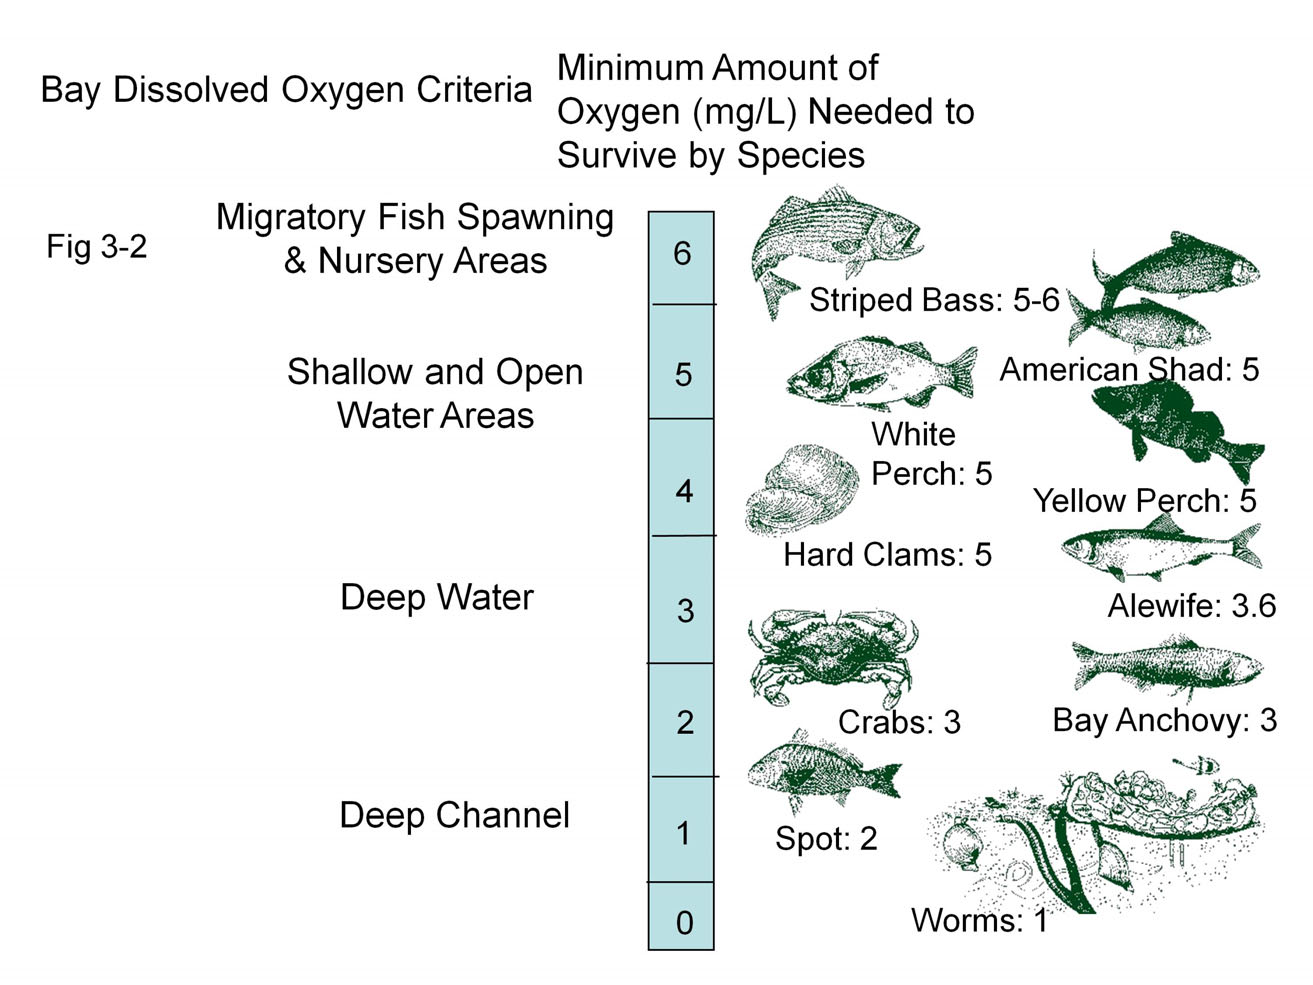
\includegraphics[height=5cm]{figs/fish_requirements.jpg}
        \caption{Requirement of DO for marine life}
    \end{figure}
\end{minipage}



DO decreases exponentially with the increase in salinity(Chi et al., 2020).

In summer and winter, the temperature differential is small between day and night, affecting the convection process and hampering the mixture of upper and lower layers of the ocean; due to this and continuous consumption of DO in the lower layers can lead to hypoxic situations.
The temperature differential is high in spring and autumn between day and night, allowing the layers to mix and keep the DO concentration consistent.

The traditional method of in-situ measurements is very time and labor-intensive, so this project aims to develop and verify a correlation between dissolved oxygen, temperature, salinity, and chlorophyll content.


% \paragraph*{}
%     Remote sensing has been an important means of monitoring dynamic changes such as rainfall, wind, temperature, etc patterns for weather monitoring and disaster forecast.

%     Dissolved oxygen(DO) is defined as the amount of free and non-compound oxygen dissolved in the water body(Chi et. al 2020)

%     Although, water quality remains an improtant element for the survial of flura and fauna, it is still monitored through in-situ monitoring stations; though, these stations provide accurate data there temporal and spatial resolution is inadquate. Hence, there is an opening
%     for satellite remote sensing to develop a method to monitor water quality.

%     One such parameter is dissolved oxygen, it is the amount of oxygen present in a water body. Water bodies receie oxygen from the atmosphere and from the aquatic plants with stagnant bodies having less content than moving ones.

%     Hence, we can extrapolate that dissolved oxygen is directly lines to the marine ecosystem and even a little change can cause a negative imapct.

%     Some literature such as Keeling et al.[2010] suggets that dissolved oxygen in open ocean has been declining in the past centuries, be it due to natural causes or increase in temperature.

%     The traditional method of in-situ measurements is very time and labour intensive, so the idea of this project is to develop and verify a correlation between dissolved oxygen, temperature, salinity, chlorophyll content.

%     Over the past severl decades, water quality retrieval by remote sensing has been widely concerned and developed rapidly (Dekker etal. 1992; Duan et al. 2012; Gons, 1999)

%     In existing research, the most focused water quality parameters include Chlorophyll-a, temperature and colored dissolved organic matter(CDM); other parameters which can be helpful for estimating dissolved oxygen are salinity, turbidity, nitrate concentration and specific conductance.


%     DO decreases expnentially with the increase in salinity(Chi et al. 2020).

%     In summer and winter, the temperature of upper layer of water body is relatively higher or lower than the lower layer(>3m) and the temperature differenece between day and night is small(Walker and Lucke, 2018). As a result the upper layer is less dense and remains at the top of the lake. The mixture of layers is cut-off but DO is consumed continuously in the lower layer which leads to DO decrease and even hypoix situations.

%     In spring and autumn, due to increas in the temperature variations, the density of upper layer is lower in daytime and higher in night, which promotes the mixture between the layers allowing the DO to remain consistant.

    \section{Data \& Methodology}
        \paragraph{}
This project aims to develop and verify a correlation between the water parameters such as chlorophyll concentration, temperature, salinity, pH, and specific concentration with Dissolved Oxygen(DO).
Therefore, we require both in-situ and remote observation to make quantitative predictions. 

Here we have utilized the USGS real-time water parameters for in-situ observations and AQUA-MODIS from NASA ocean color(NASA OBPG) as the remote dataset, discussed in section II.I and II.II respectively.

For analyzing and predicting the dissolved oxygen concentration, a multiple regression model is developed using the data from 2018-01-01 to 2021-12-31, discussed in section II.III

        \subsection{In-situ data: USGS WaterQualityWatch}
            \paragraph{Introduction}
    USGS provides an almost real-time environment to gather multiple parameters from water in/nearby the United States, i.e., water temperature, pH, salinity, and specific conduction.
    
    It provides the data in tab-separated \textit{.rdb} files with more information about the format available at \href{https://help.waterdata.usgs.gov/faq/about-tab-delimited-output}{waterdata.usgs.gov}.

    \begin{figure}[H]
        \centering
        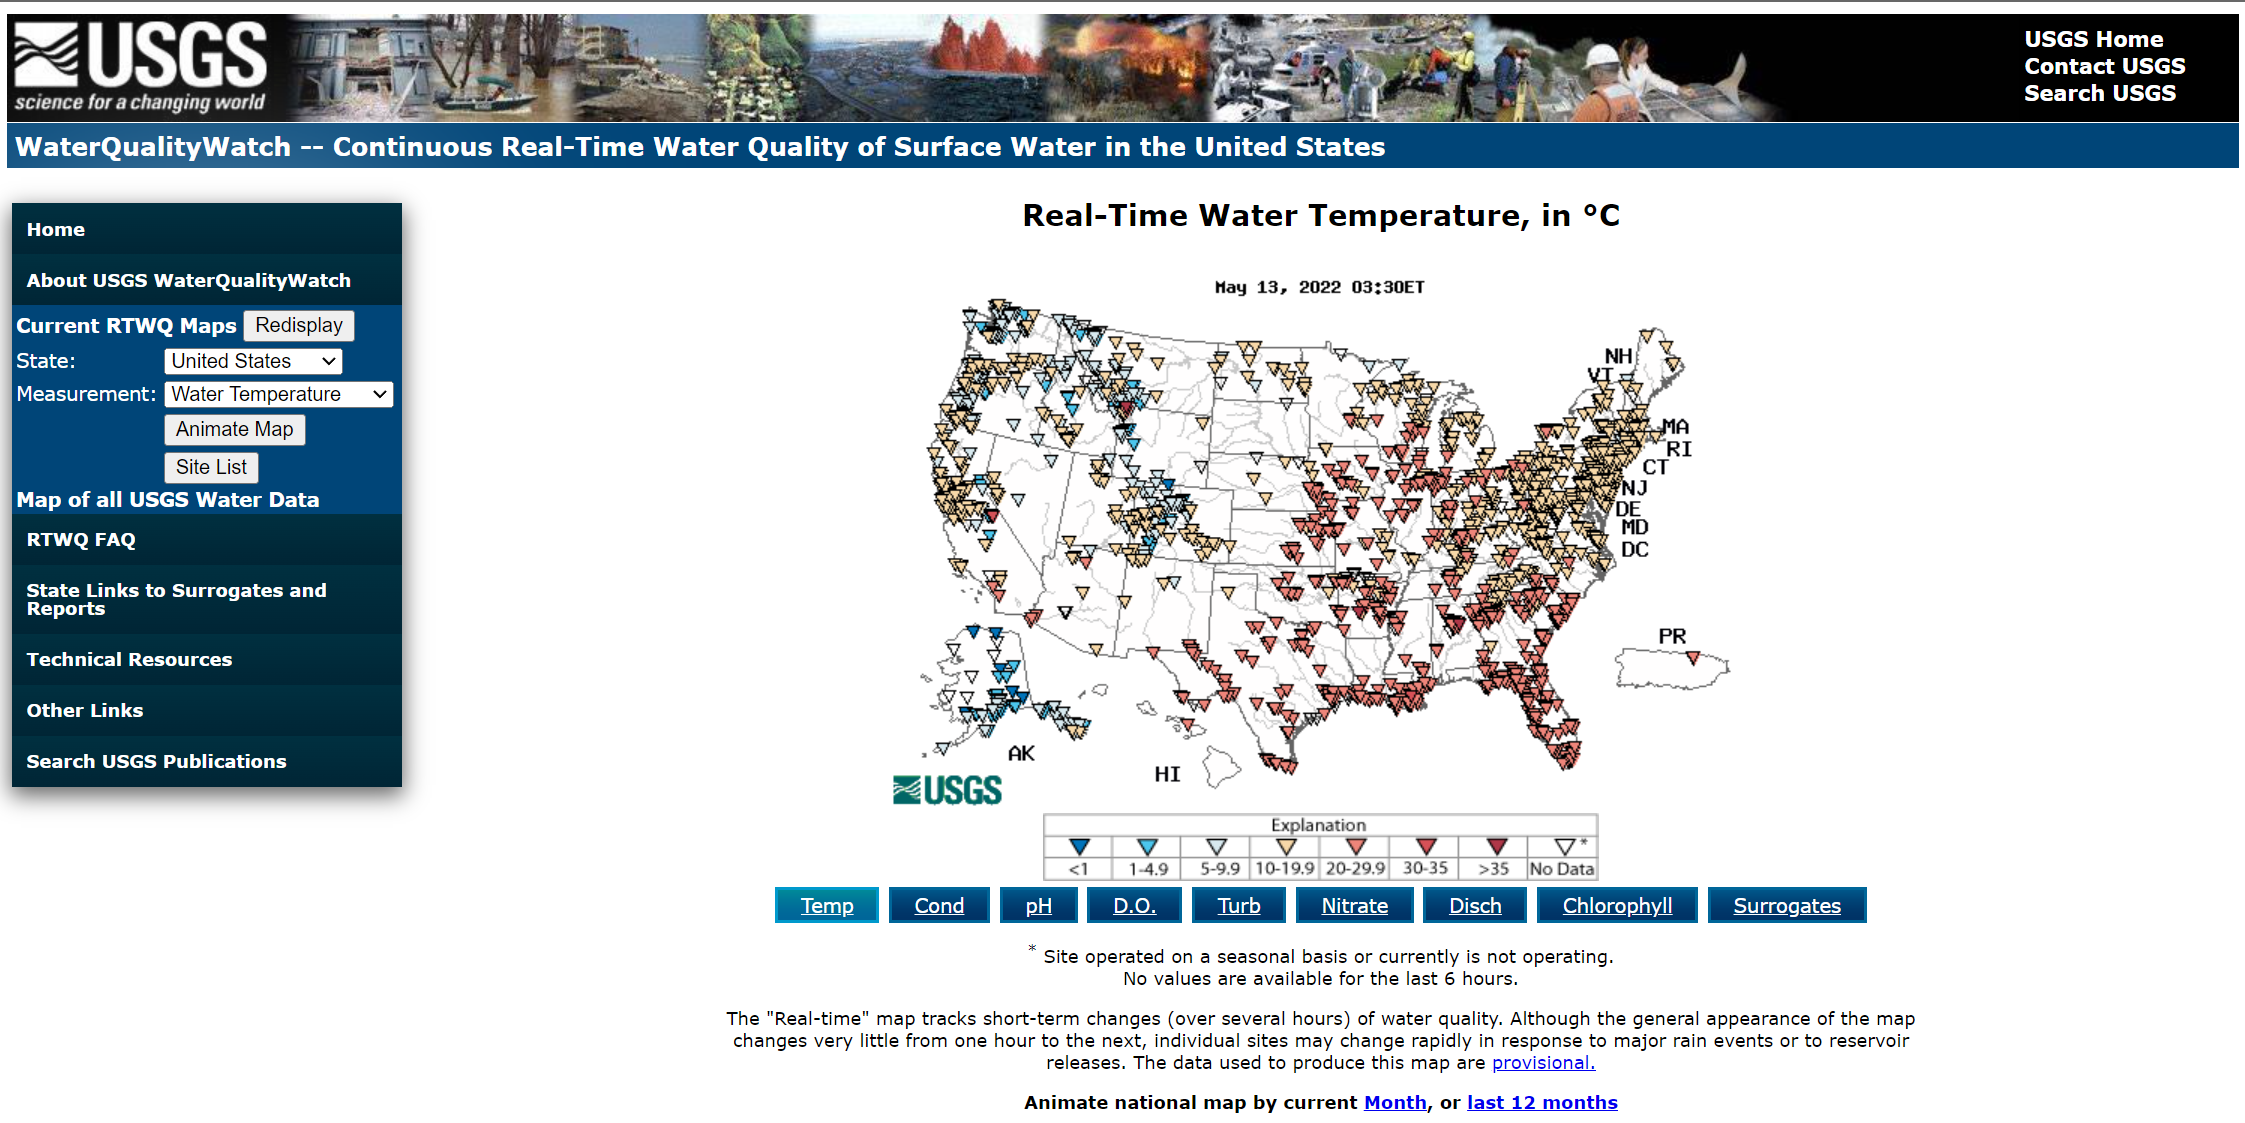
\includegraphics[scale=0.30]{figs/usgs_water.png}
        \caption{USGS WaterQualityWatch stations}
    \end{figure}

\paragraph{Data processing}
    The location chosen for analysis is \textit{ORIENT HARBOR AT ORIENT NY}, located at $41.13663889^\circ N$ and $-72.30675^\circ E$, accurate to $\pm .1 s$

    The rationale behind choosing this location was the easy availability of data for 2018-01-01 to 2021-12-31 and its closeness to the Atlantic ocean.

    Its closeness to the Atlantic ocean made it easy to obtain the subset of data from the ocean color dataset of Sea Surface Temperature(\textit{SST}) and Chlorophyll(\textit{Chlor\_a})

    \begin{figure}[H]
        \centering
        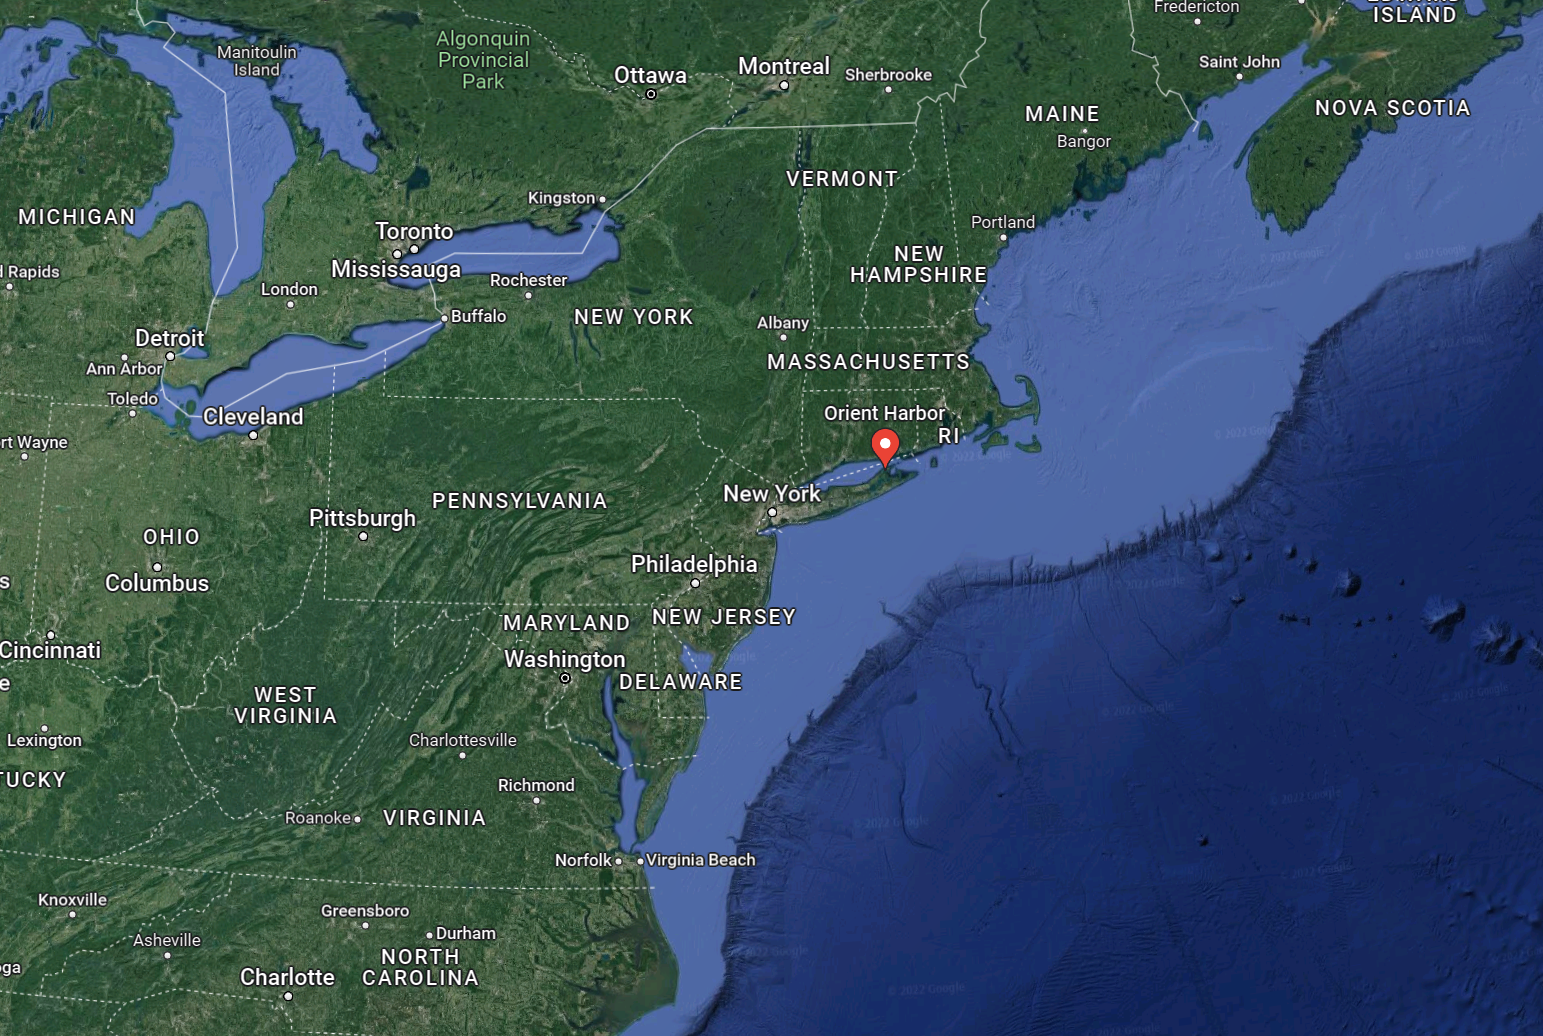
\includegraphics[width=10cm]{figs/RSS_SATELLITE_OBS.png}
        \caption{Satellite blown-up view}
    \end{figure}
    \begin{figure}[h]
        \centering        
        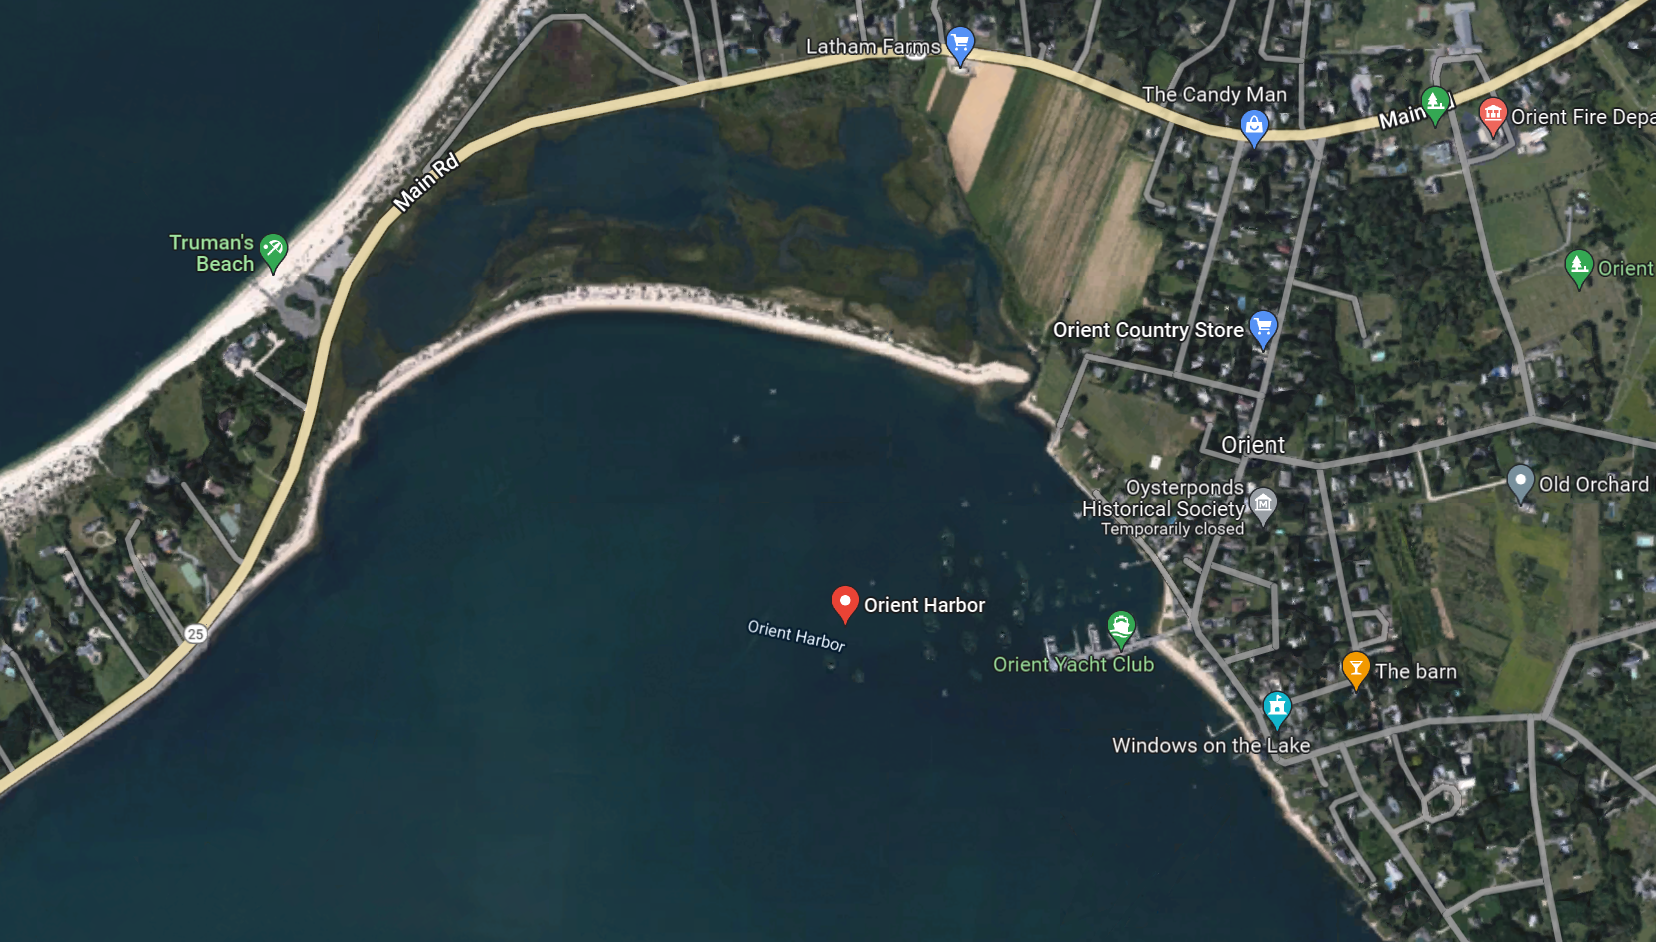
\includegraphics[width=10cm]{figs/RSS_OBS.png}
        \caption{Satellite close-up view}
    \end{figure}
    
    \paragraph{NOTE:}
    For better results and analysis choosing multiple locations with adequate separation would be ideal, but the turbidity and water contamination may bias our analysis, so we have restricted to a single location as a proof-of-concept.

        \subsection{Remote data: Aqua-MODIS}
            \begin{figure}[H]
    \subfloat[MODIS external]{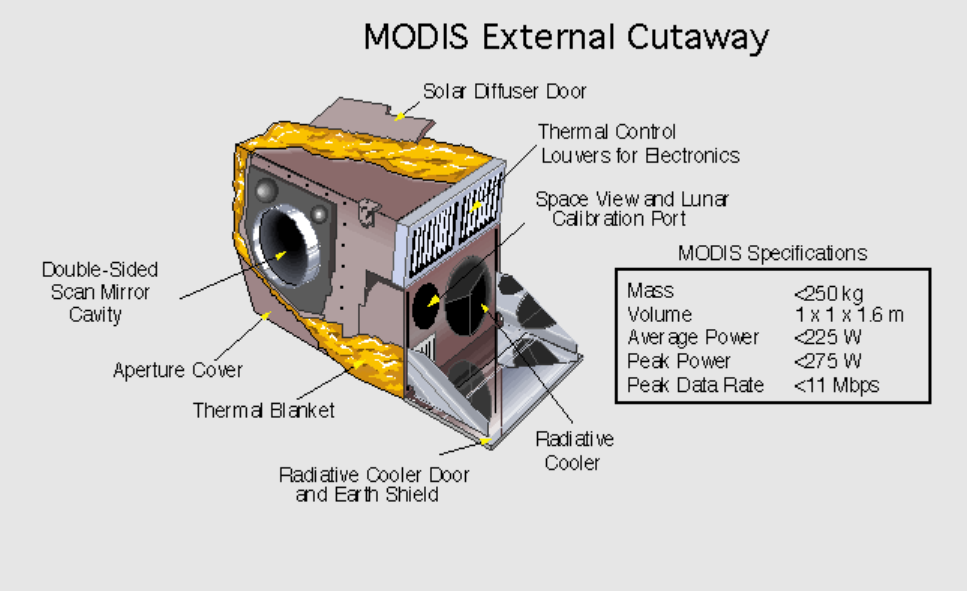
\includegraphics[scale=0.45]{figs/MODIS-external.png}}
    \quad
    \subfloat[MODIS subsystems]{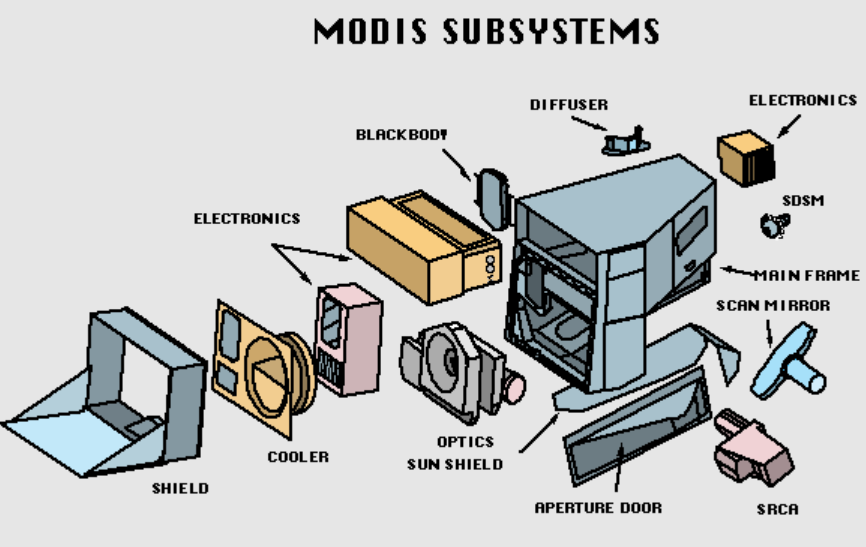
\includegraphics[scale=0.5]{figs/modis-sub.png}}
    \caption{MODIS (credits: wikipedia.org)}
\end{figure}
\paragraph{Introduction}
MODIS (or Moderate Resolution Imaging Spectroradiometers) is an instrument onboard the Terra(EOS AM)
and Aqua(EOS PM) satellites. Terra's orbit around the Earth is timed so that it passes from north to south
across the equator in the morning, while Aqua passes south to north over the equator in the afternoon. MODIS
is designed to provide measurements in large-scale global dynamics, including oceans, land, and cloud cover.
The Scan Mirror Assembly uses a continuously rotating double-sided scan mirror to scan $\pm55$-degrees and is
driven by a motor encoder built to operate at 100 percent duty cycle throughout the 6-year instrument design
life

\begin{figure}
    \centering
    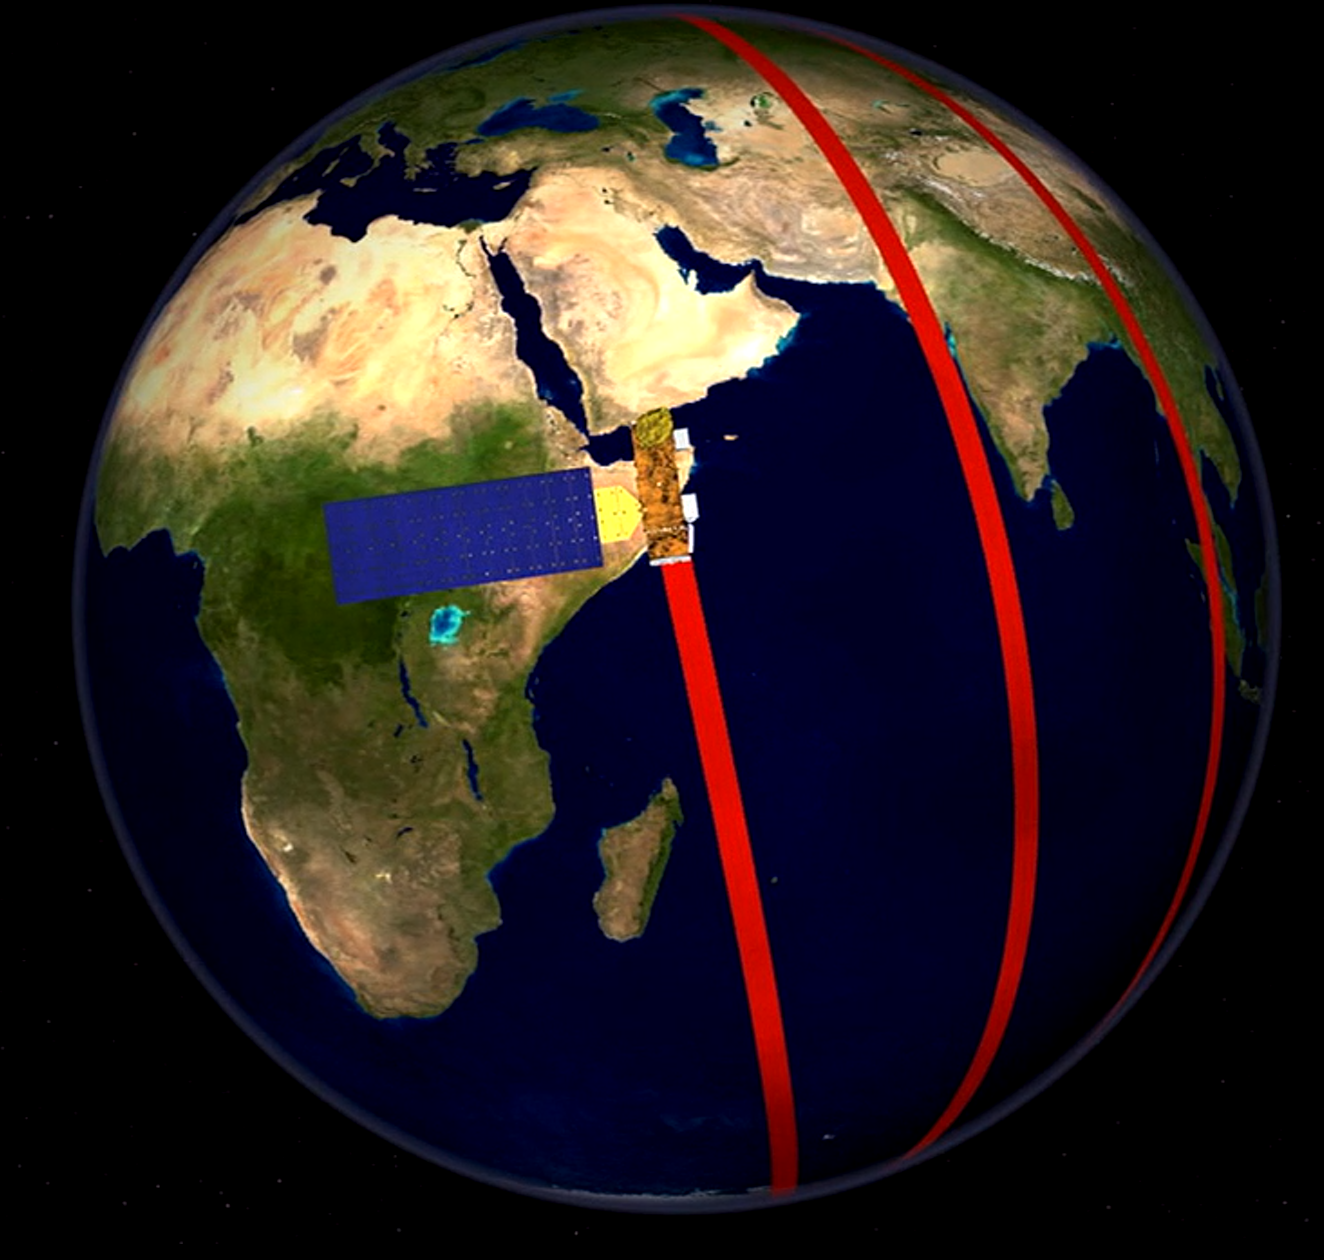
\includegraphics[scale=0.25]{figs/aqua_orbit.png}
    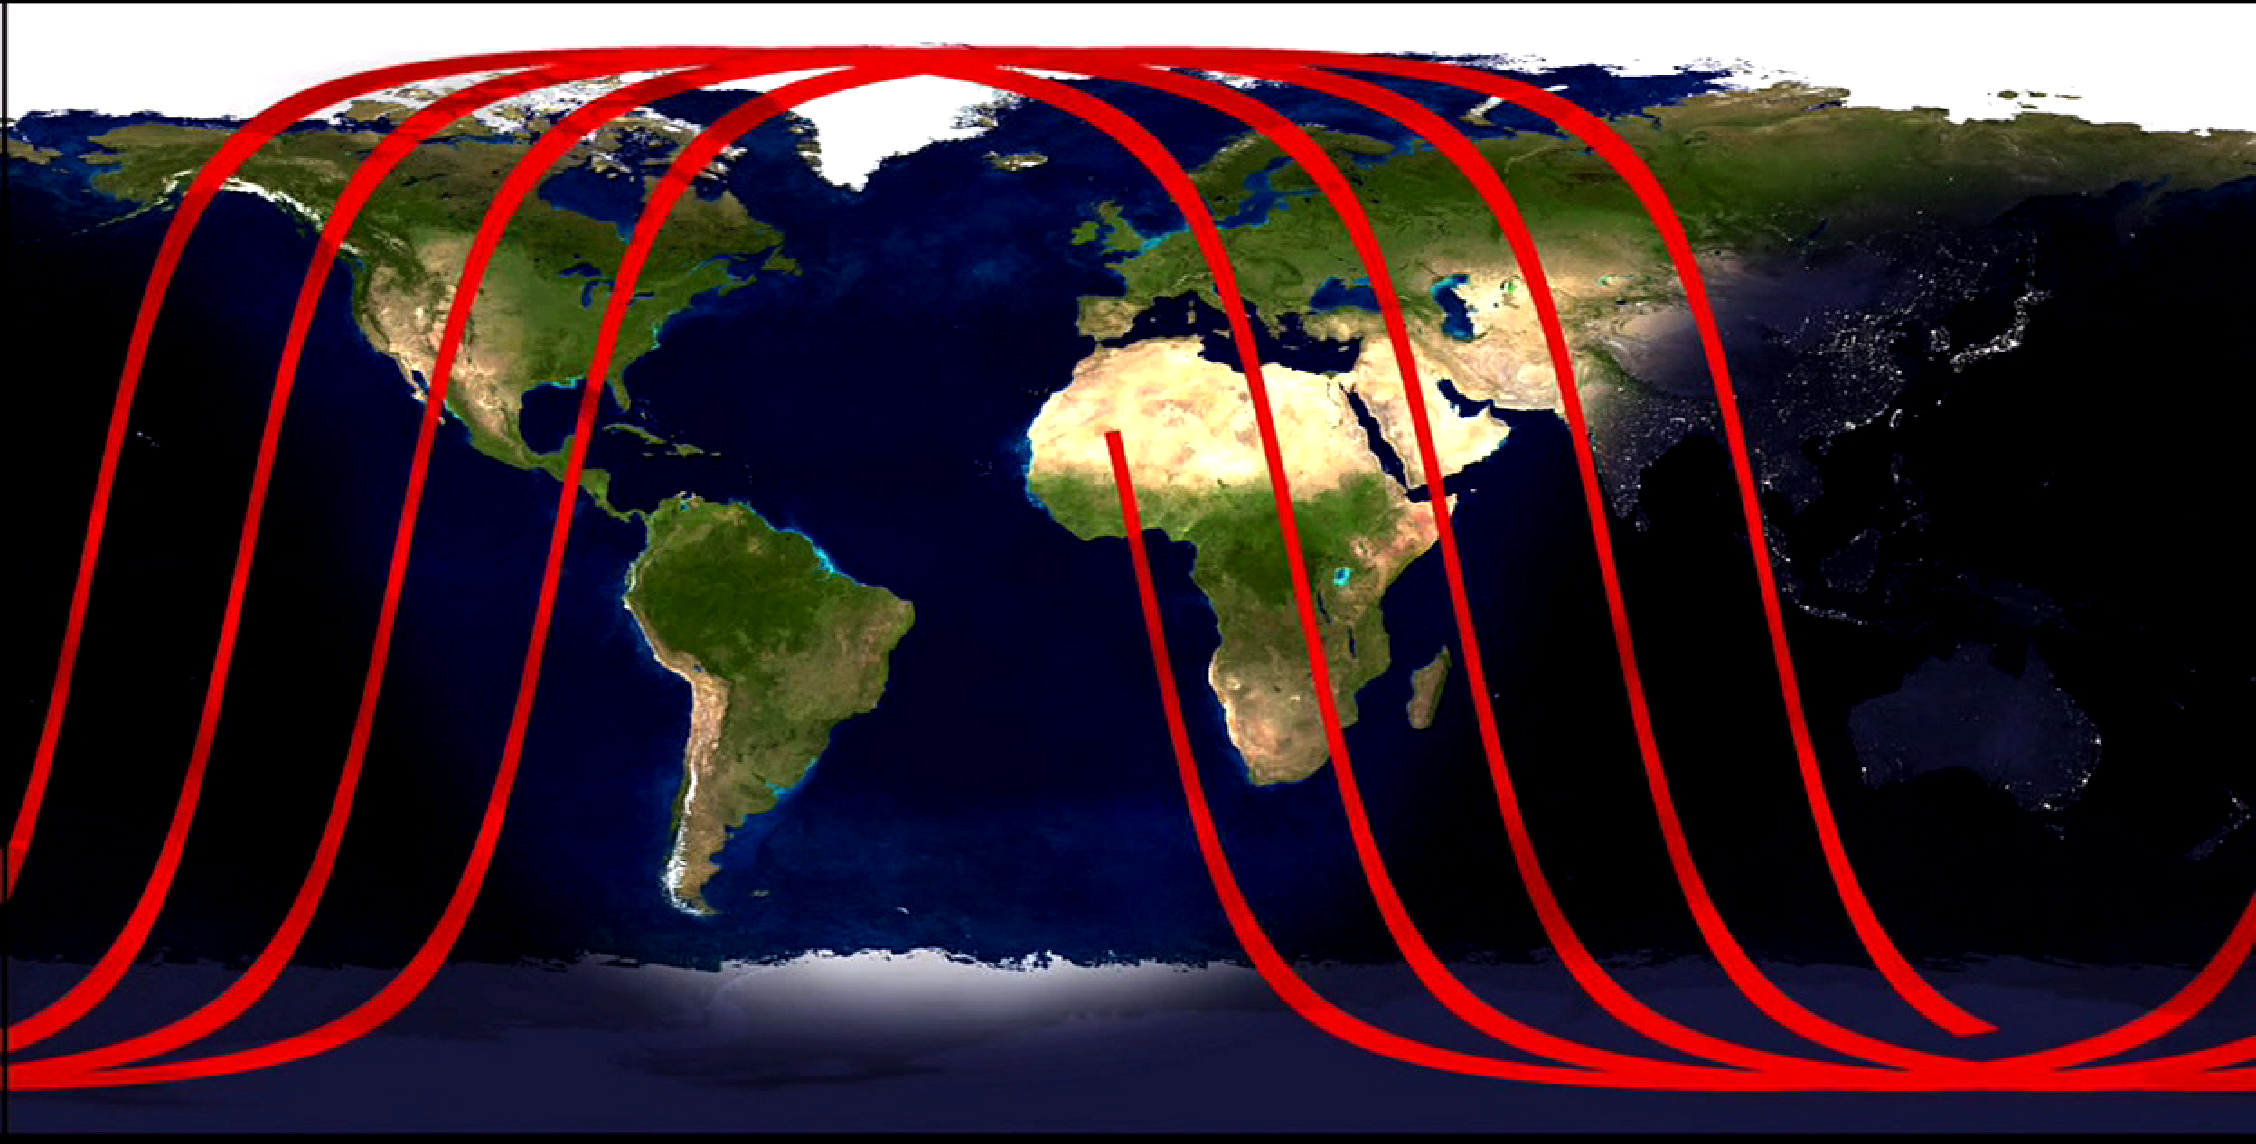
\includegraphics[scale=0.25]{figs/aqua_orbit2.png}
    \caption{AQUA-MODIS orbit, credits:NASA GSFC}
\end{figure}

\paragraph{Specification}
It captures 36 spectral bands ranging in wavelength from $0.4\mu m$ to $14.4\mu m$ and at varying spatial resolutions.
Together the instruments image the entire Earth every 1 to 2 days.
It has a sun-synchronous, near-polar orbit of 705km with a swath of 2300km cross-track by
10km along the track at nadir. It has a scan rate of 20.3rpm cross track.
MODIS's temporal resolution is 1-2 days and was launched and designed to work for at least 6-years.


\paragraph{Data processing}
    \subsubsection{Sea Surface Temperature (SST)} The Sea surface temperature is observed at $11\mu m$ and $4\mu m$ for day and night respectively with $4km$ and $9km$ spatial resolution.
    In this analysis, we have utilized the $11\mu$ with $4km$ resolution daily data.

    \begin{figure}[H]
        \centering
        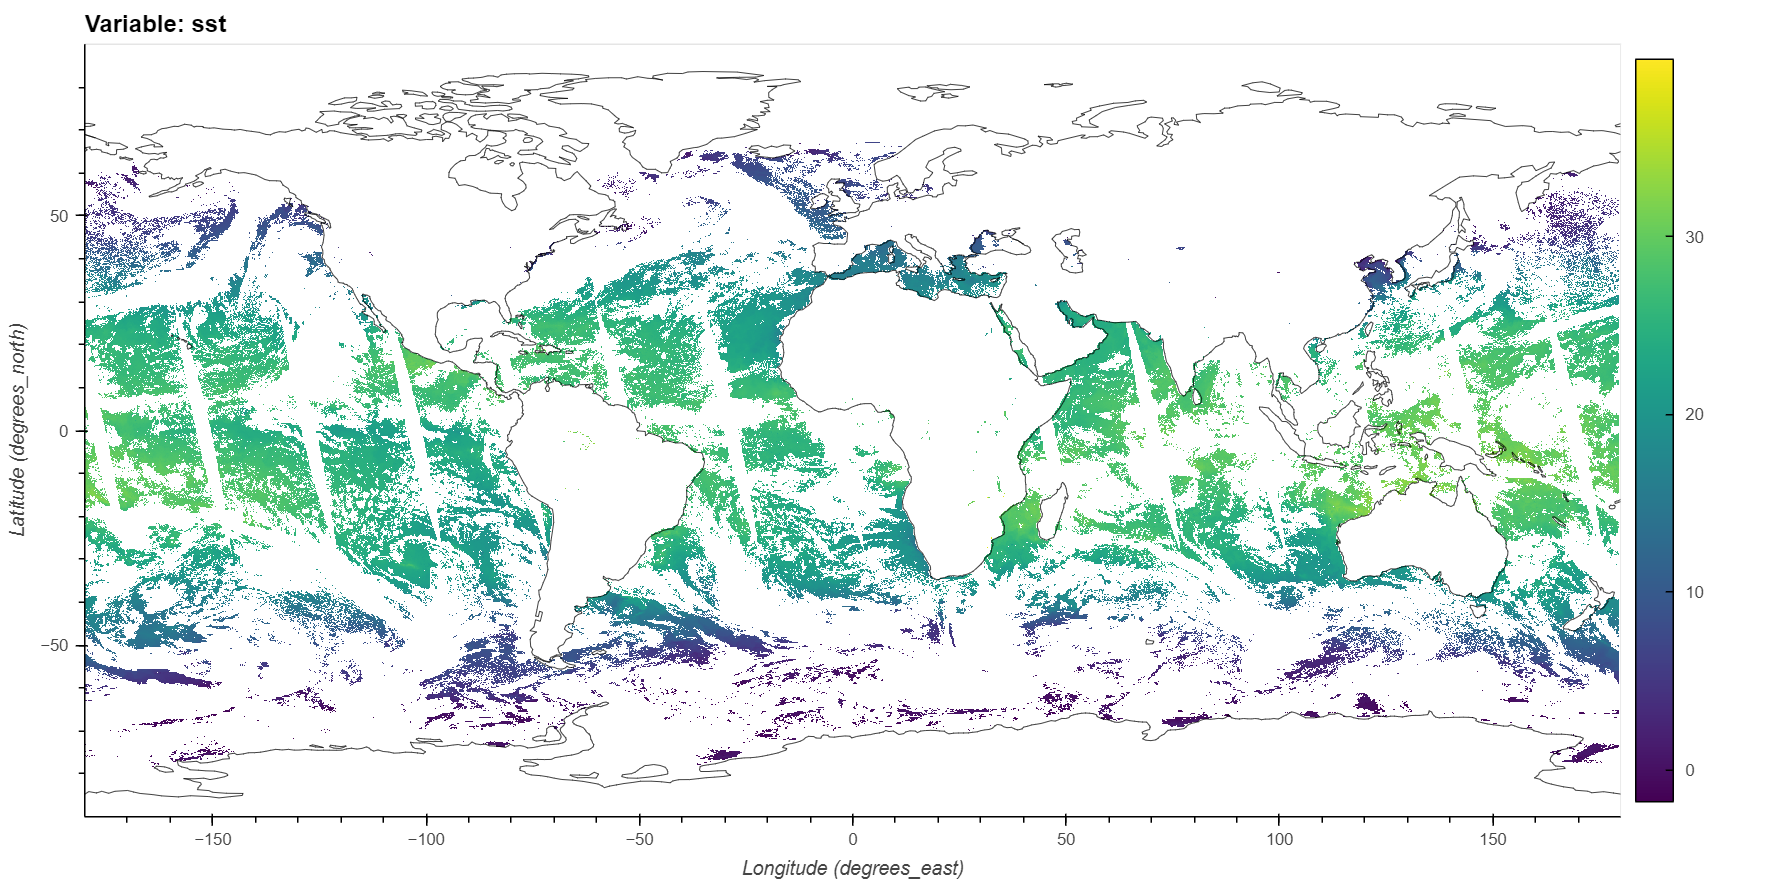
\includegraphics[width=\textwidth]{figs/sst_20180101.png}
        \caption{Sea Surface Temperature($^\circ C$; $11\mu$) 2018/01/01}
        {\footnotesize Processed and plotted in python with using `nctoolkit`;}
        {\footnotesize the white portions represent land mass, swaths and cloud cover.}
    \end{figure}

    \begin{figure}[H]
        \centering
        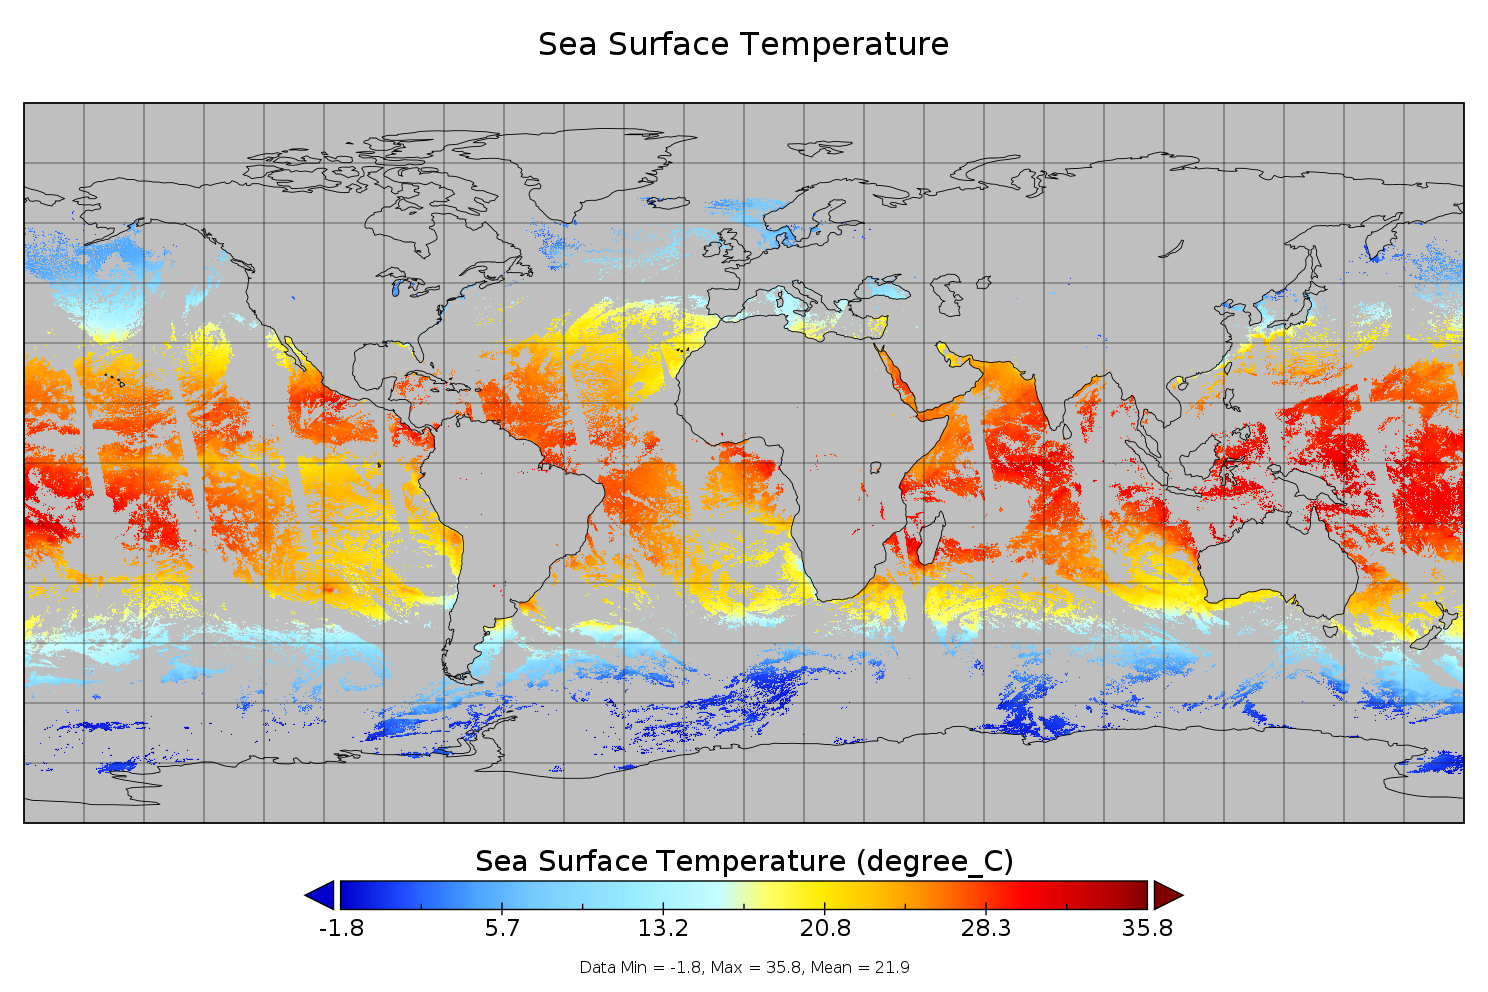
\includegraphics[width=14cm, trim={{0cm} {0.5cm} {0cm} {0cm}}, clip]{figs/sst_in_AQUA_MODIS_20180102.png}
        \caption{Sea Surface Temperature($^\circ C$; $11\mu$) 2018/01/02}
        {\footnotesize Processed and plotted using NASA Panoply with interpolations enabled}
    \end{figure}

    \paragraph{Monthly averaged}
        The daily fluctuations vanishes when we average for a month; the remaining fluctuations are called monthly temperature anamolies.

        \begin{figure}[H]
            \centering
            \includegraphics[width=\textwidth]{figs/AQUA_MODIS_20180101_20180131.png}
            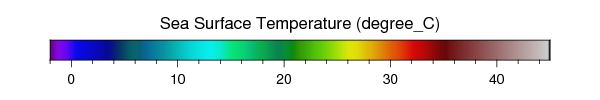
\includegraphics[scale=0.4]{figs/sst_colorbar.png}
            \caption{Montly averged temperatures for January 2018}
        \end{figure}
    
    \subsubsection{Chlorophyll} The chlorophyll content cannot be directly measured using remote methods, so in this analysis the chlorophyll-A is computed using the NASA OCI algorithm.

    This algorithm returns the near-surface concentration of Chlorophyll-A(chlor\_a) in $mg\; m^{-3}$, calculated using an empirical relationship derived from in-situ measurements of chlor\_a and remote sensing reflectances ($R_{rs}$) in the blue-to-green region of the visible spectrum.

    In this analysis, we have utilized the $4km$ spatial resolution daily dataset.

    \begin{figure}[H]
        \centering
        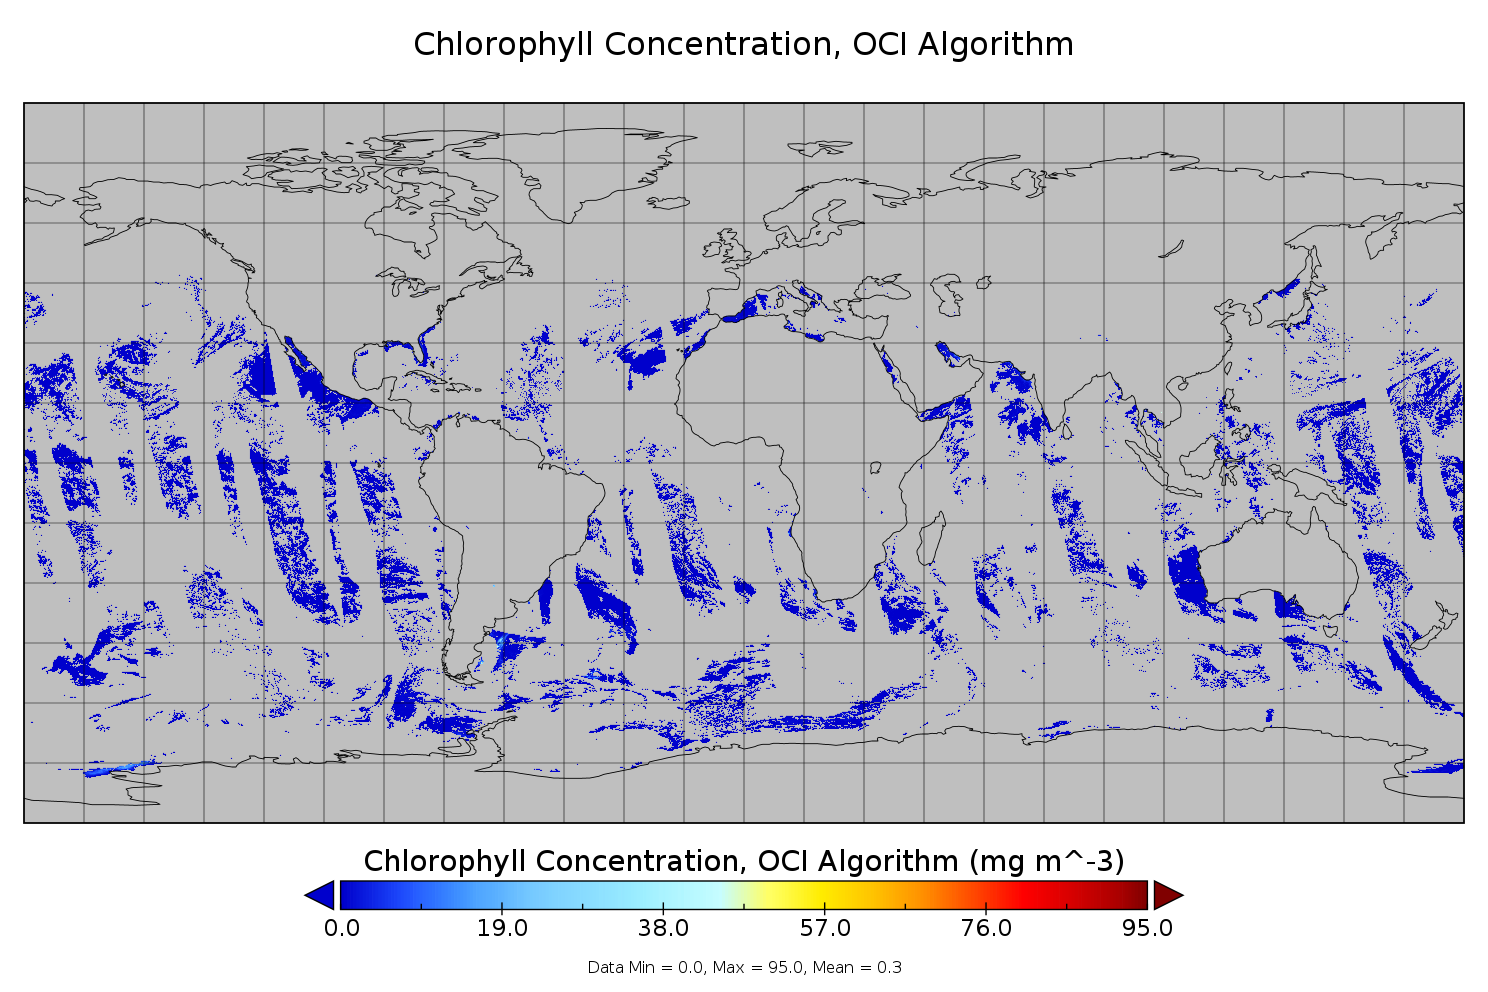
\includegraphics[width=14cm, trim={{0cm} {0.5cm} {0cm} {0cm}}, clip]{figs/chlor_a_in_A2018004.png}
        \caption{Chlorophyll-A 2018/01/04}
        {\footnotesize Processed and plotted using NASA Panoply with interpolations enabled}
    \end{figure}
    
    \begin{figure}[H]
        \centering
        \includegraphics[width=14cm]{figs/A20180012018031png.png}
        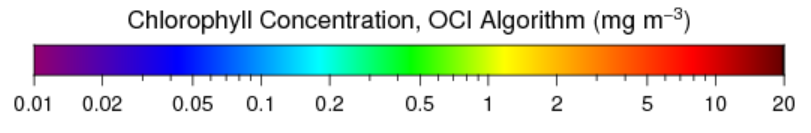
\includegraphics[scale=0.4]{figs/chl_colorbar.png}
        \caption{Montly averged chlorophyll-a (OCI) for January 2018}
    \end{figure}

% \begin{table}[H]
%     \centering
%     \begin{tabular}{l|c|c|c}
%         \toprule\toprule
%         Band & wavelength(nm) & Spatial resolution(m) & Spectral width(nm) \\
%         \midrule
%         Band 1 - Red & $620-670$ & $250$ & $2.0$ \\
%         Band 2 - NIR & $841-876$ & $250$ & $6.0$ \\
%         Band 3 - Blue/Green & $459-479$ & $500$ & $6.0$ \\
%         Band 4 - Green & $545-565$ & $500$ & $3.0$ \\
%         Band 5 - NIR & $1230-1250$ & $500$ & $8.0$ \\
%         Band 5 - mid IR & $1628-1652$ & $500$ & $18.0$ \\ 
%         Band 5 - mid IR & $2105-2155$ & $500$ & $18.0$ \\
%         \bottomrule
%     \end{tabular}
% \end{table}
        \subsection{Methodology}
            \paragraph{}
    The in-situ data source is \textit{ORIENT HARBOR AT ORIENT NY}, but the remote data is worldwide with 4km resolution. Therefore, we limit our remote data to a polygon around the monitoring station.
    To reduce complexity, we choose this polygon to be a box with a latitudes range of $[40, 41.250] ^\circ N$ and a longitudes range of $[-73, -71]^\circ E$; this box encompasses an area of $25000\;km^2$ (refer to Fig 8).

    The remote data subset is spatial averaged to account for fluctuations inside the box.

\begin{figure}[H]
    \centering
    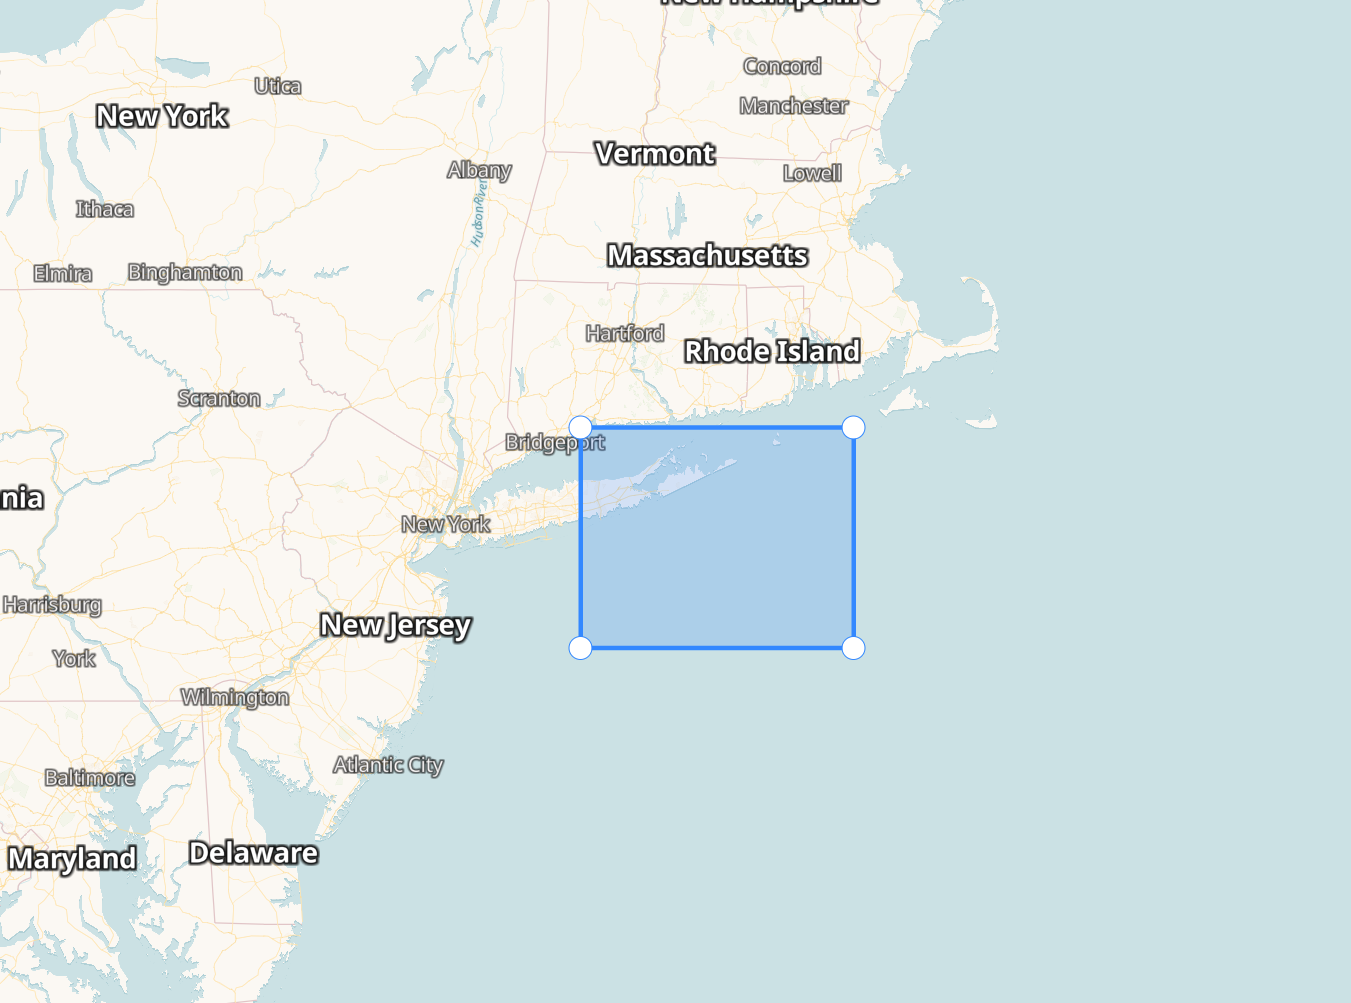
\includegraphics[scale=0.5]{figs/RSS_BOX.png}
    \caption{Subset for remote data}
\end{figure}


\paragraph*{}
    After gathering the data, we use the supervised machine learning algorithm called the \textbf{Multiple Linear Regression} to develop a relationship.
    \begin{equation}
        y = \beta_0 + \beta_1 x_1 + \beta_2 x_2 + \cdots + \beta_n x_n
    \end{equation}

    We have utilized pH, salinity, field temperature, remote temperature and specific conductance as our input parameters, so our equation will become
    \begin{equation}
        DO = \beta_0 + \beta_1 pH + \beta_2 (\text{salanity}) + \beta_3 (\text{field temperature}) + \beta_4 (\text{MODIS SST}) + \beta_5 (\text{specific conductance})
    \end{equation}

    We split our dataset into two sets, labeled for supervised learning and unlabled data for testsing with $0.8$ and $0.2$ ratio respectively.
    
    \section{Analysis}
        \subsection{Field data}
Time-series data for field data from \textit{ORIENT NY} monitoring station; the data is collected at intervals of 6mins, with no data available represented by $NaN$.

As represented in Fig.\ref{fig:time_series_ny_temp}, the temperature shows a seasonal pattern at a frequency of 6-8 months, representing the gap between summer and winter seasons. Other parameters pH, dissolved oxygen, specific conductance and salinity also
follows a similar pattern with frequency around 6-months.


\begin{figure}[H]
    \hspace*{4cm}\subfloat[Temperature]{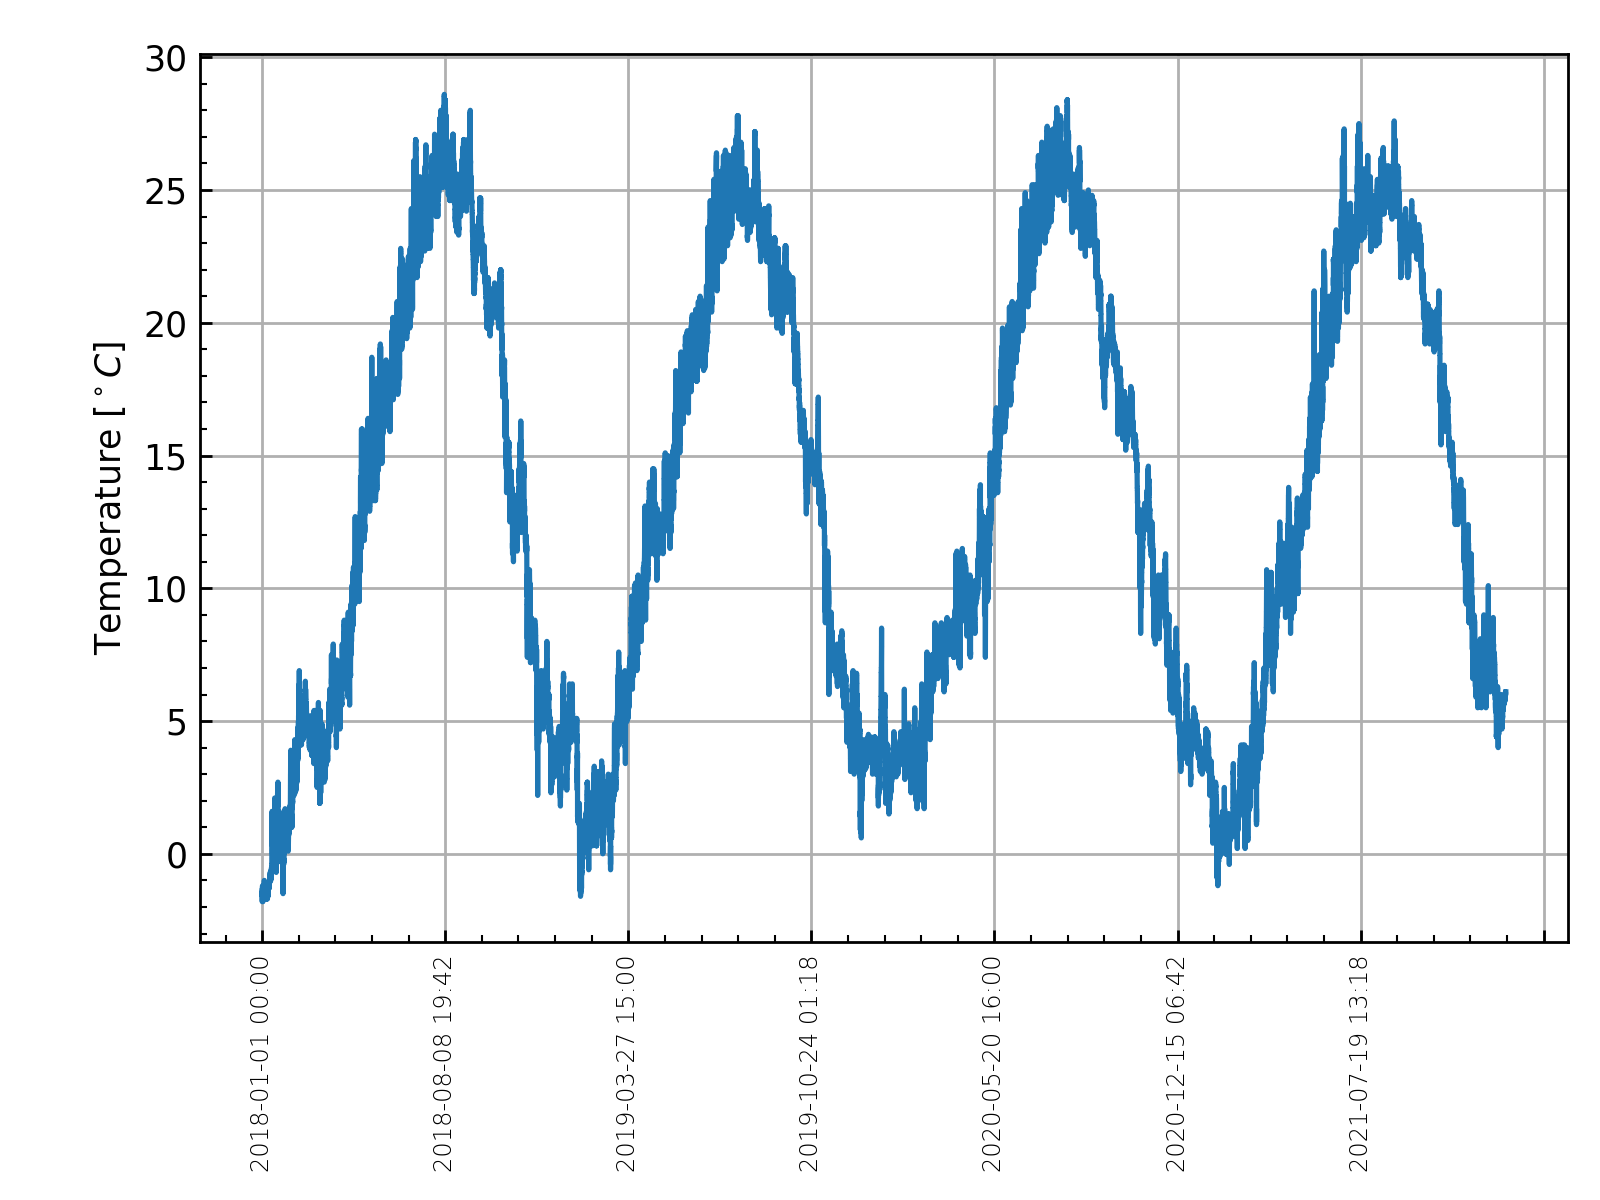
\includegraphics[scale=0.5]{figs/plots/temperature.png}\label{fig:time_series_ny_temp}} \\
    \subfloat[pH]{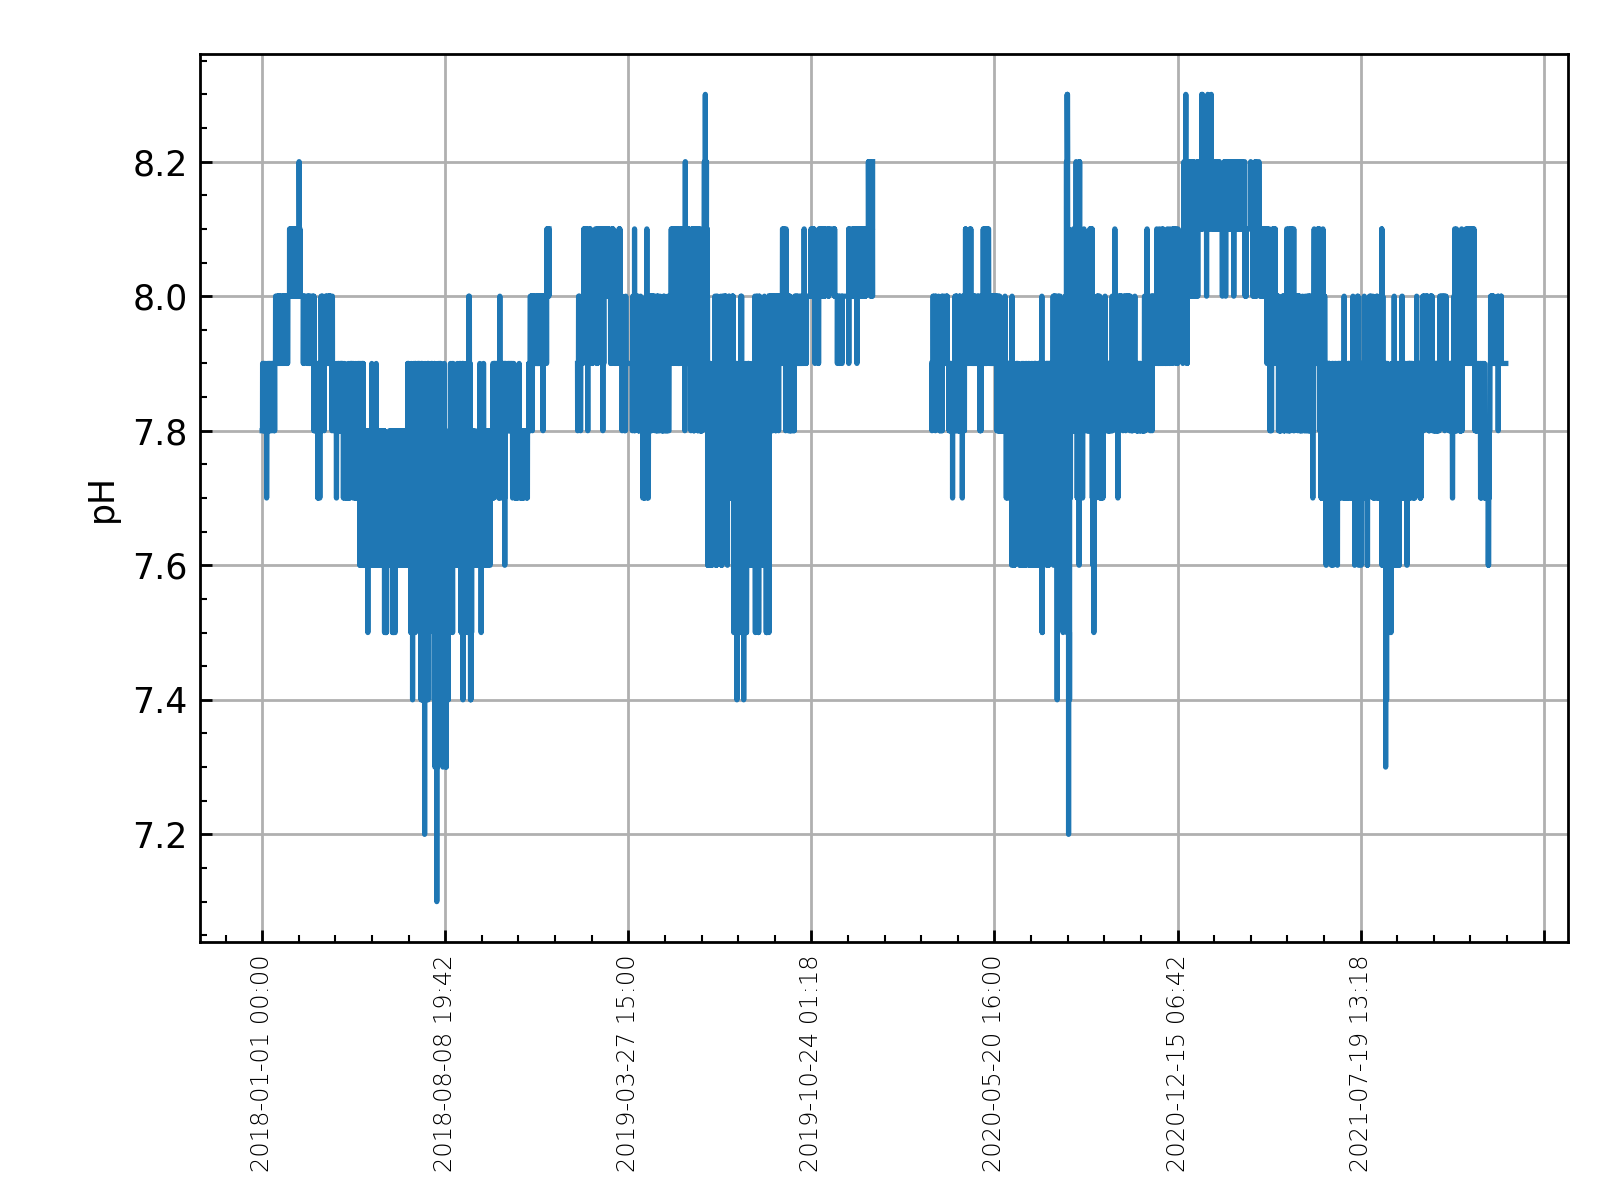
\includegraphics[scale=0.5]{figs/plots/pH.png}}
    \quad
    \subfloat[Dissolved oxygen(mg/L)]{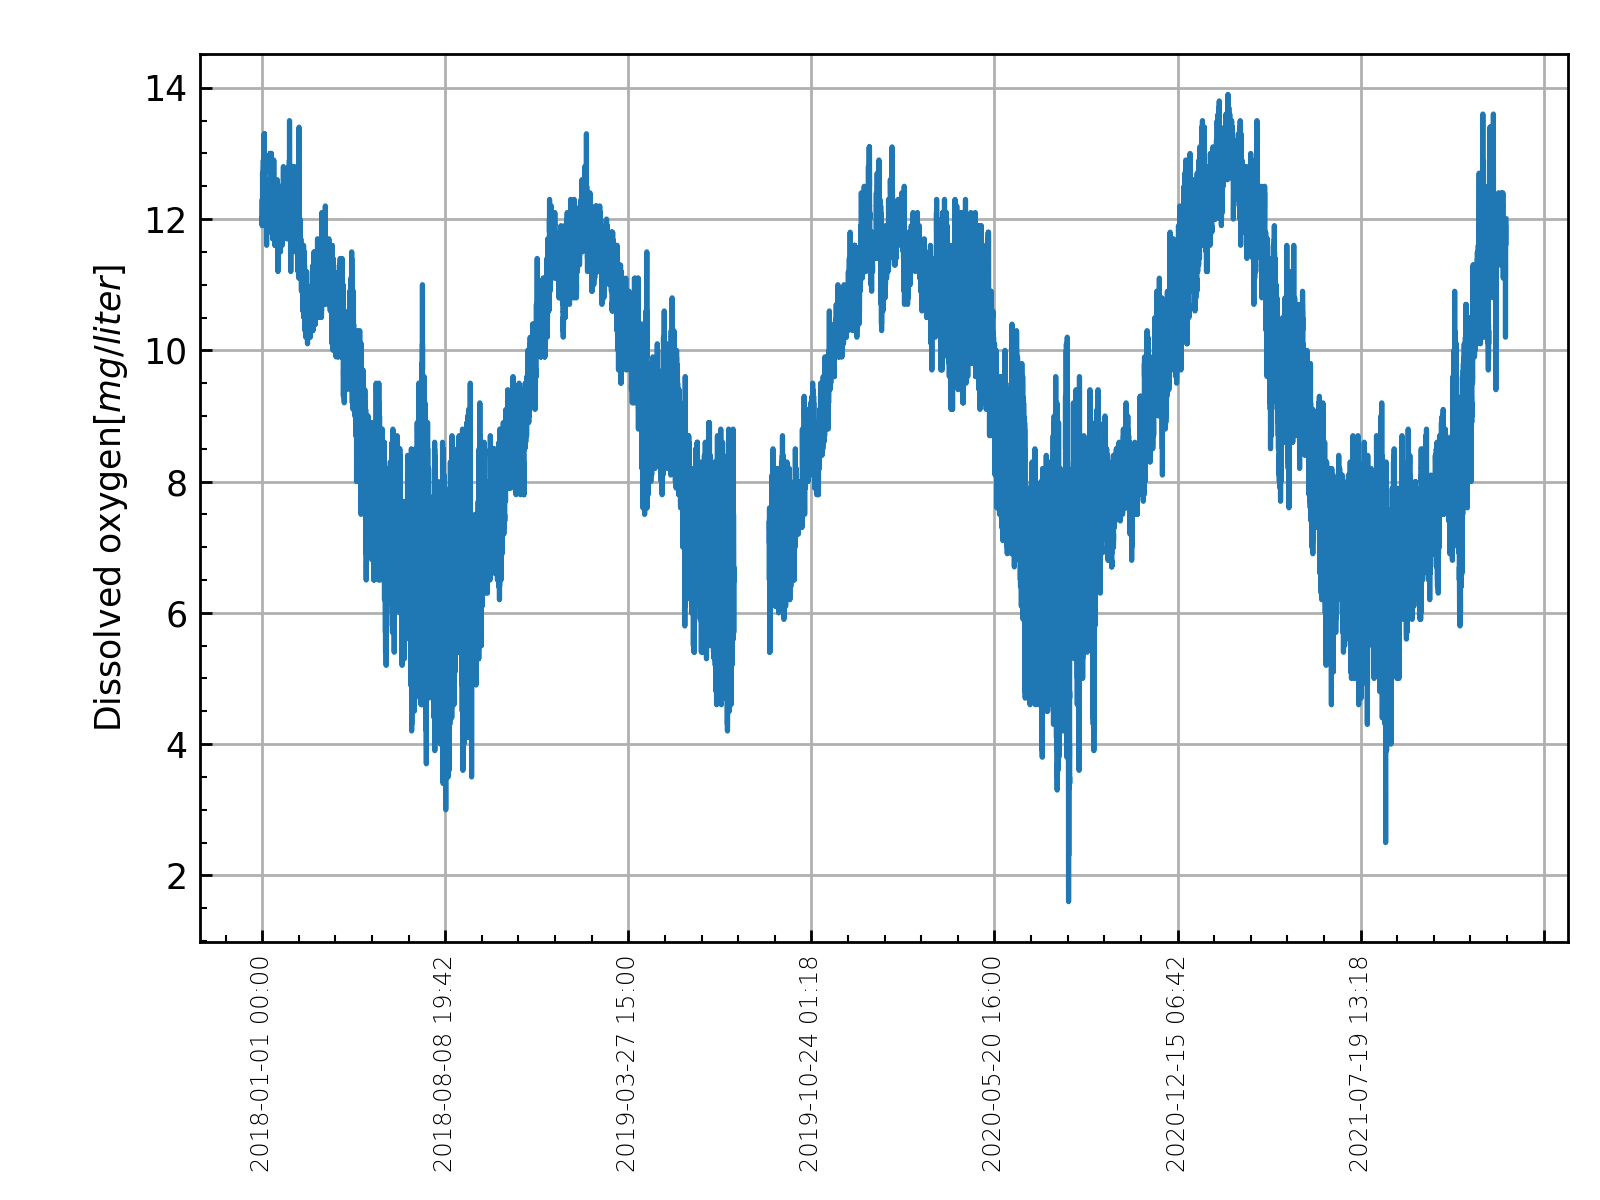
\includegraphics[scale=0.5]{figs/plots/do.png}\label{fig:time_series_ny_do}}
    \hfill
    \subfloat[Specific conductance($\mu S/cm$)]{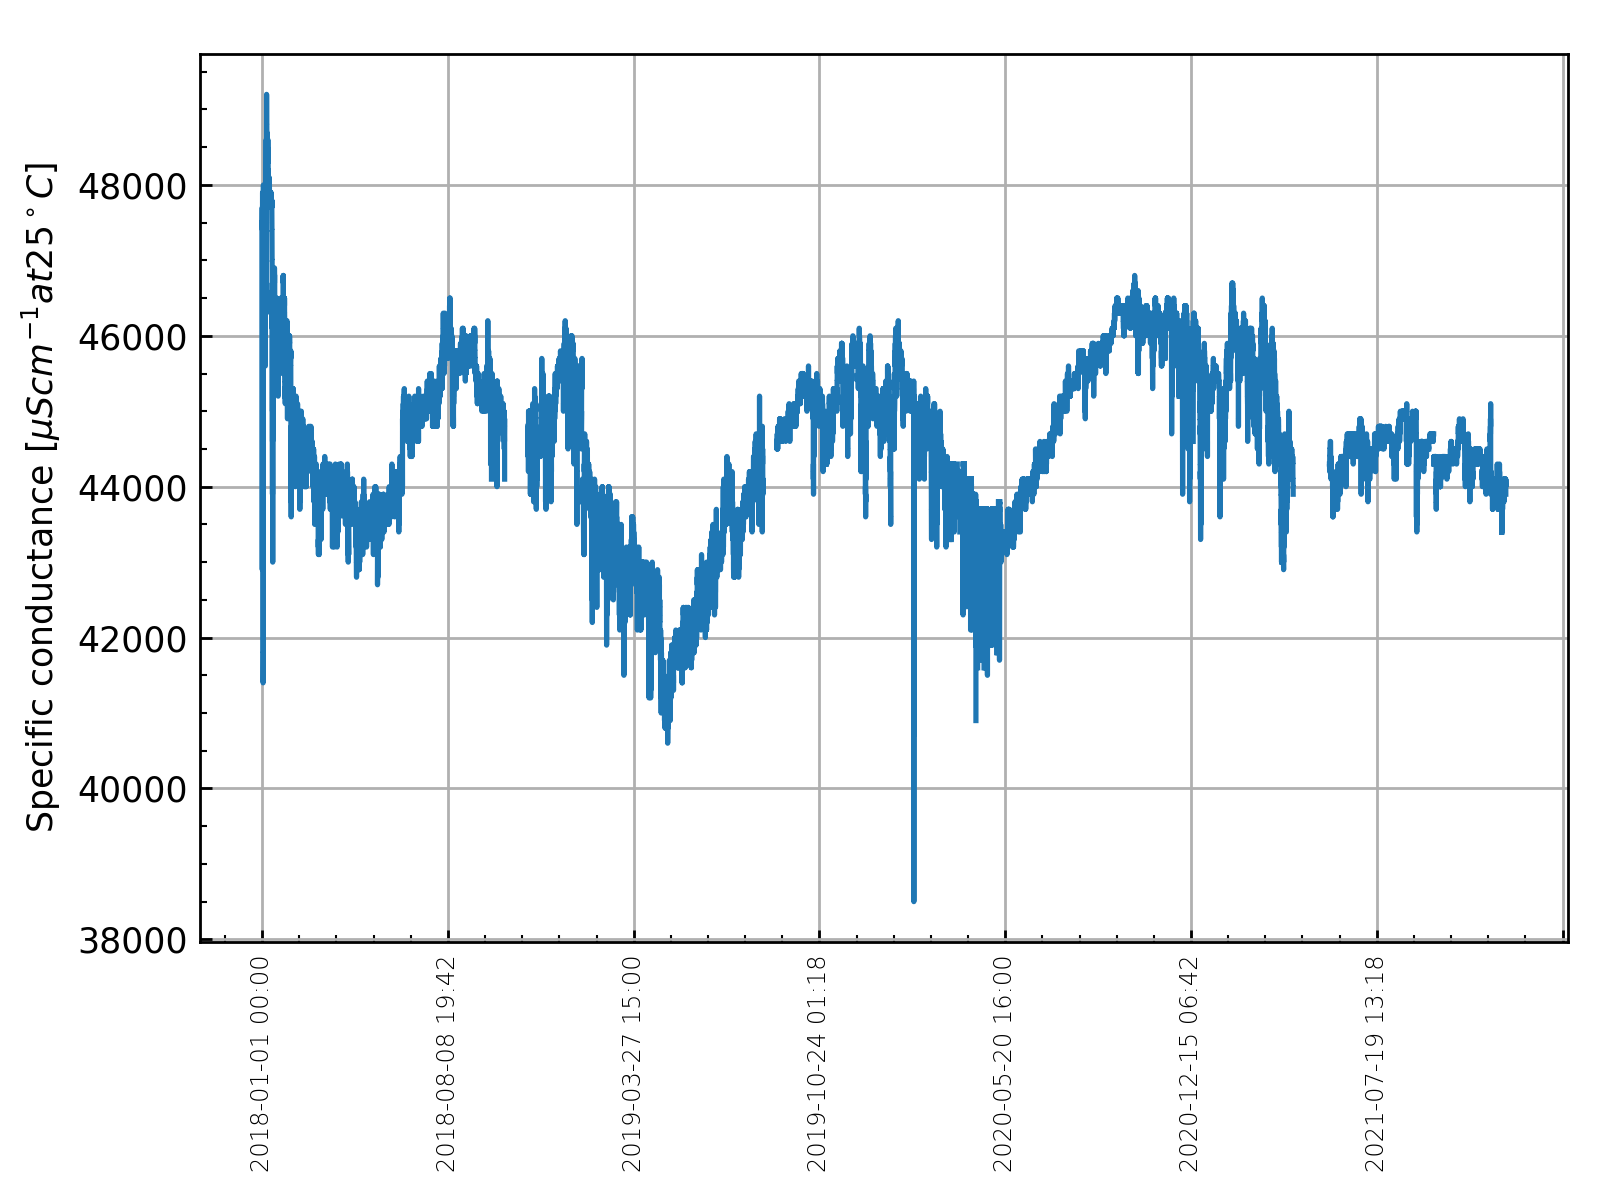
\includegraphics[scale=0.5]{figs/plots/conductance.png}}
    \quad
    \subfloat[Salinity($psu$)]{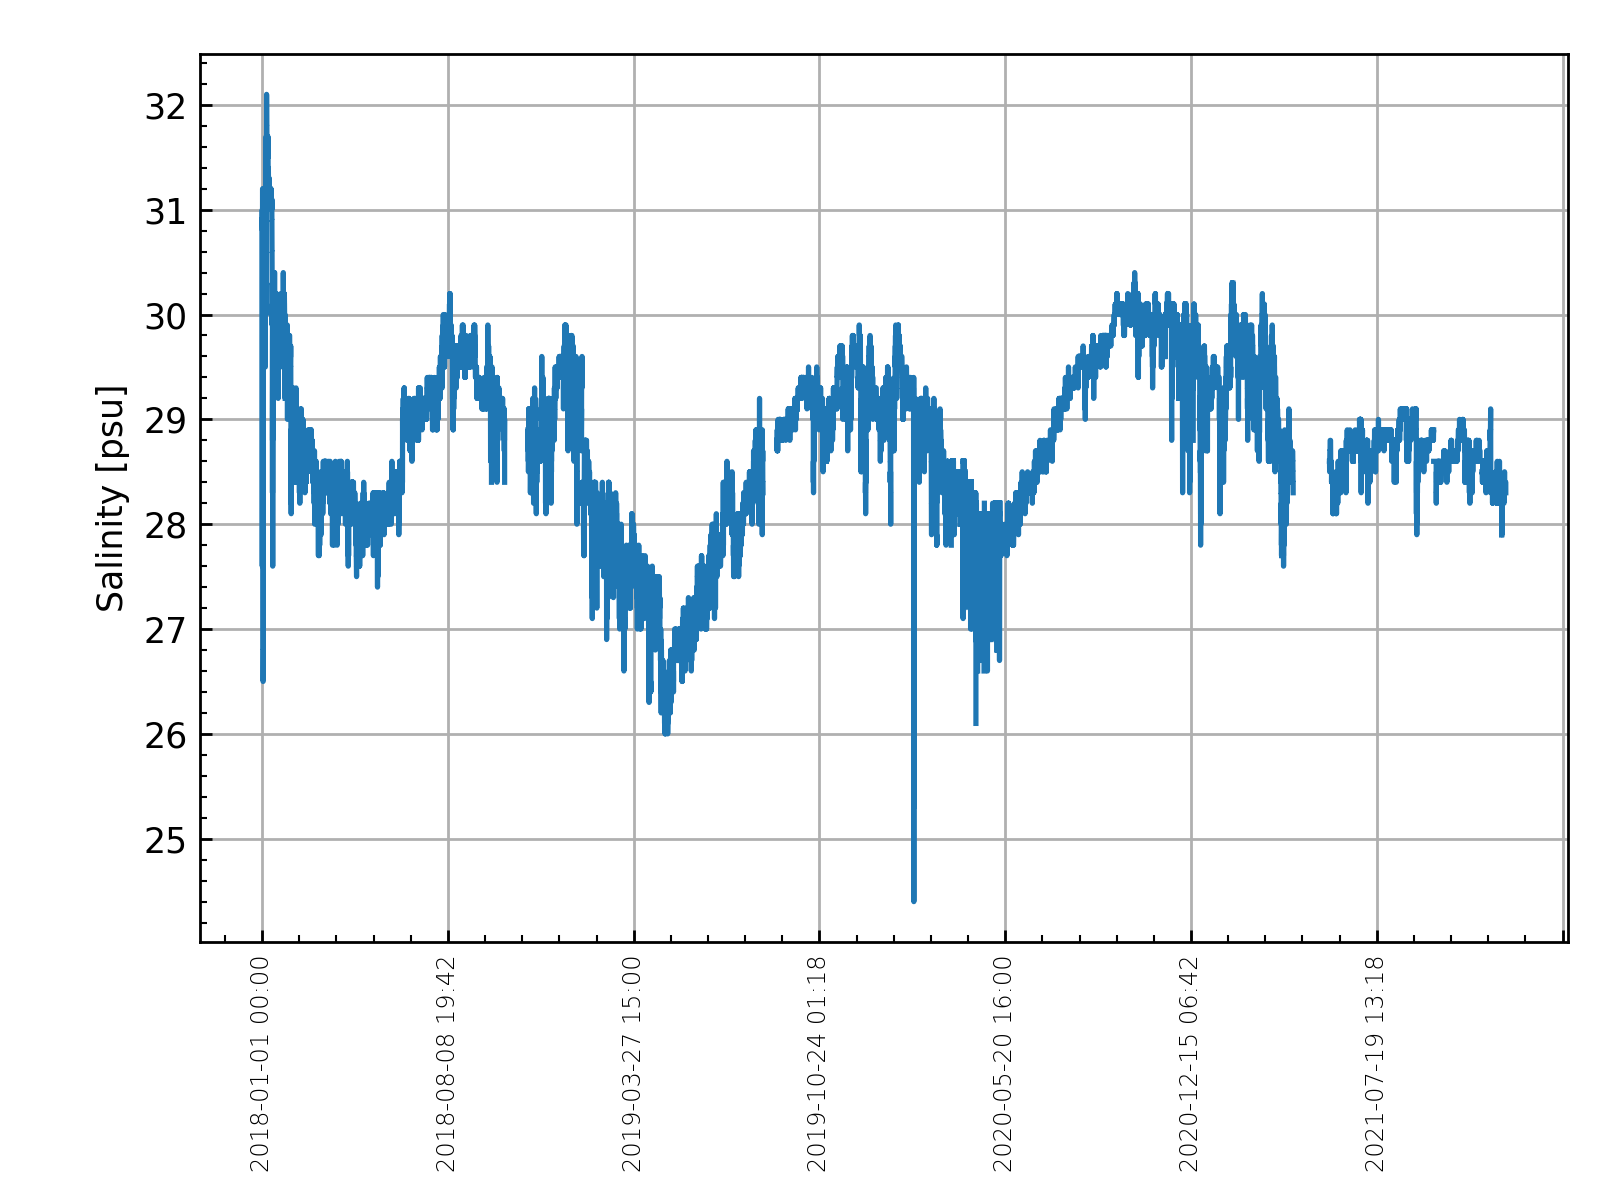
\includegraphics[scale=0.5]{figs/plots/salinity.png}}
    \caption{Orient Harbour New York, US}
\end{figure}

\paragraph{Correlation with dissolved oxygen}
By using our field data we can compute correlations matrices to solidfy our understanding of correlations between dissolved oxygen and pH, dissolved oxygen and specific conductance et al.

Through these correlation matrices we can verify that our parameters have a positive correlation with the concentration of dissolved oxygen.

\begin{figure}[H]
    \subfloat[Dissolved oxygen and salinity]{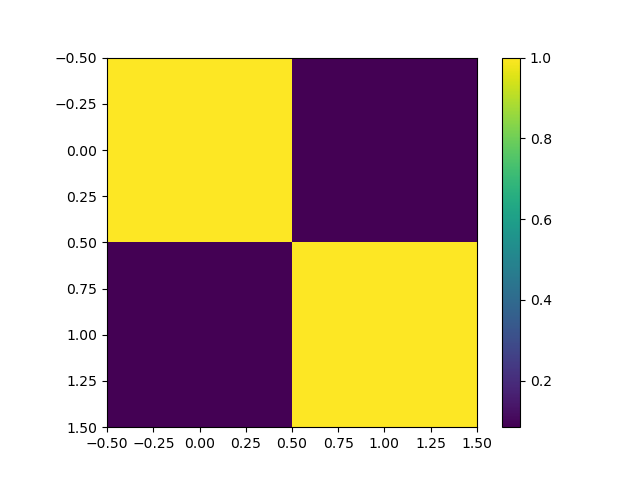
\includegraphics[scale=0.5]{figs/plots/do_vs_salinity.png}}
    \quad
    \subfloat[Dissolved oxygen and temperature]{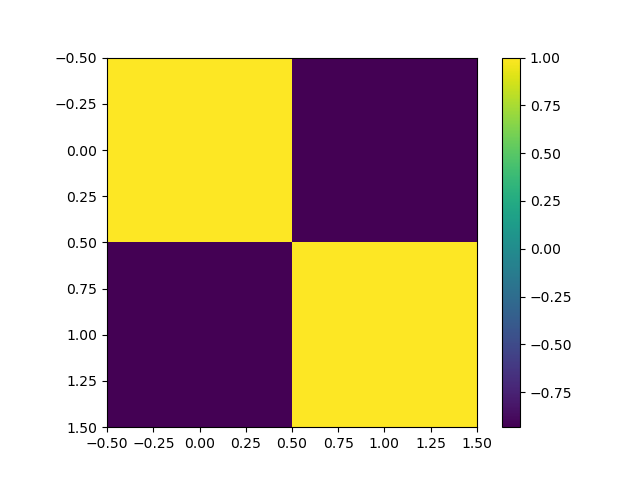
\includegraphics[scale=0.5]{figs/plots/do_vs_temp.png}}
    \hfill
    \subfloat[Dissolved oxygen and specific conductance]{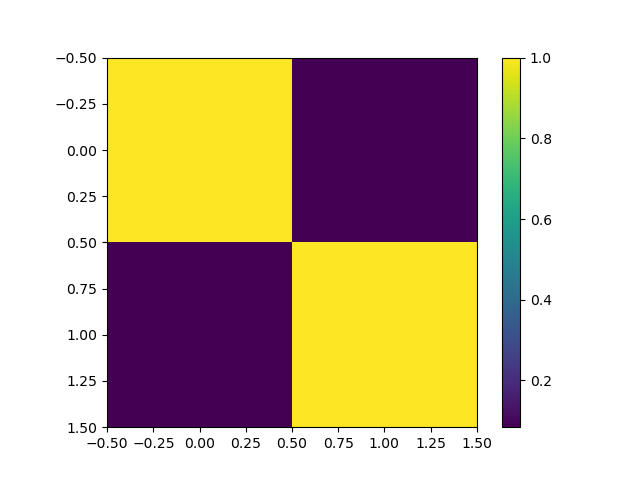
\includegraphics[scale=0.5]{figs/plots/do_vs_conductance.png}}
    \quad
    \subfloat[Dissolved oxygen and pH]{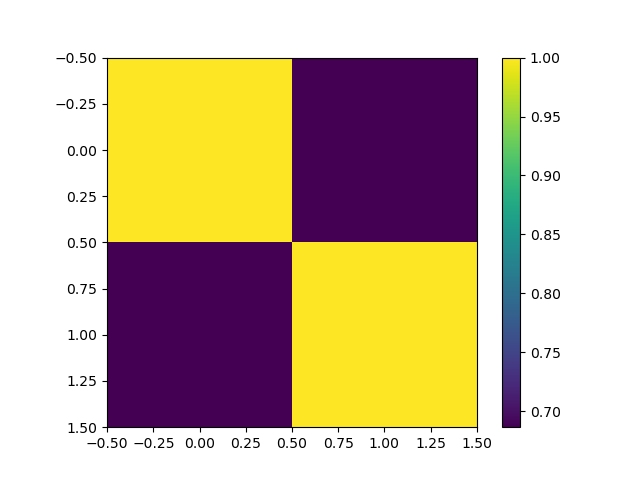
\includegraphics[scale=0.5]{figs/plots/do_vs_pH.png}}
    \caption{Correlation matrics with dissolved oxygen}
\end{figure}



\subsection{AQUA-MODIS data}
    Fig.15 represents the time-series data from the spatially averged AQUA-MODIS dataset for SST and Chlorophyll-A for our geofenced location of \textit{ORIENT NY}

\begin{figure}[H]
    \subfloat[SST($11\mu m$; $^\circ C$)]{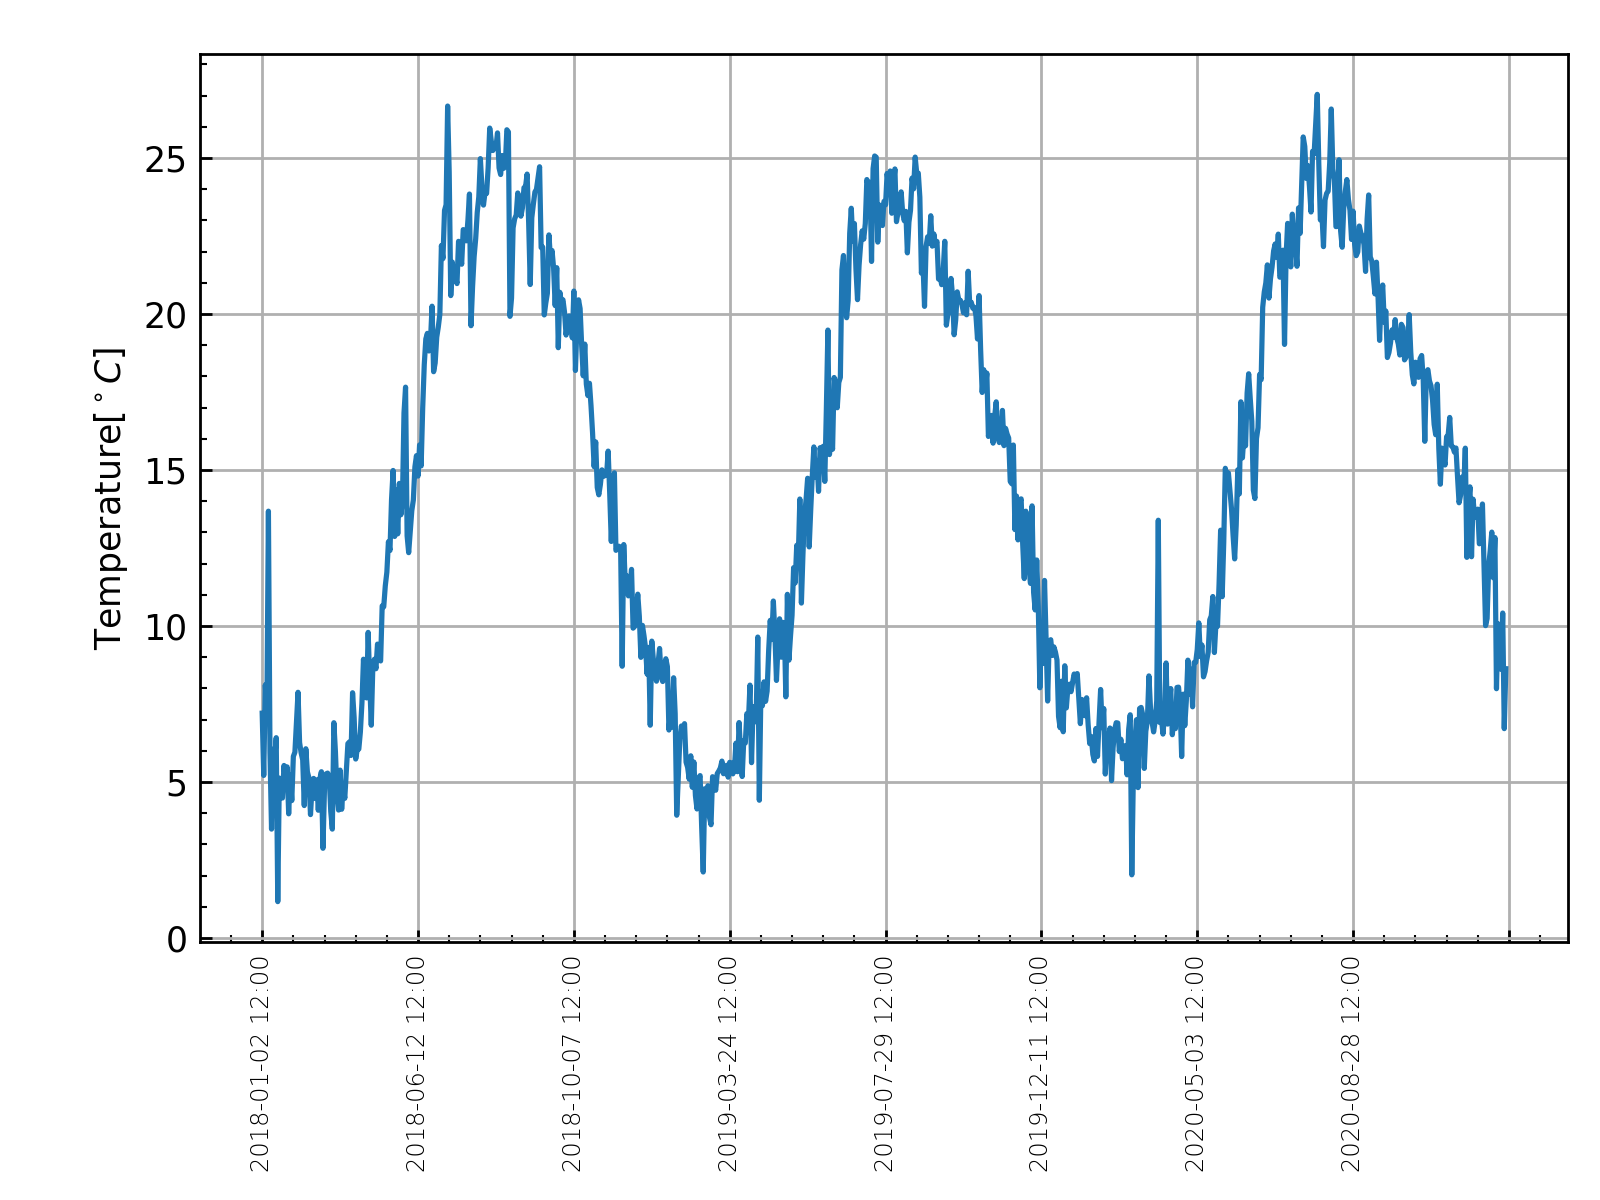
\includegraphics[scale=0.5]{figs/plots/sst.png}}
    \quad
    \subfloat[Chlorophyll-A($mg/m^3$)]{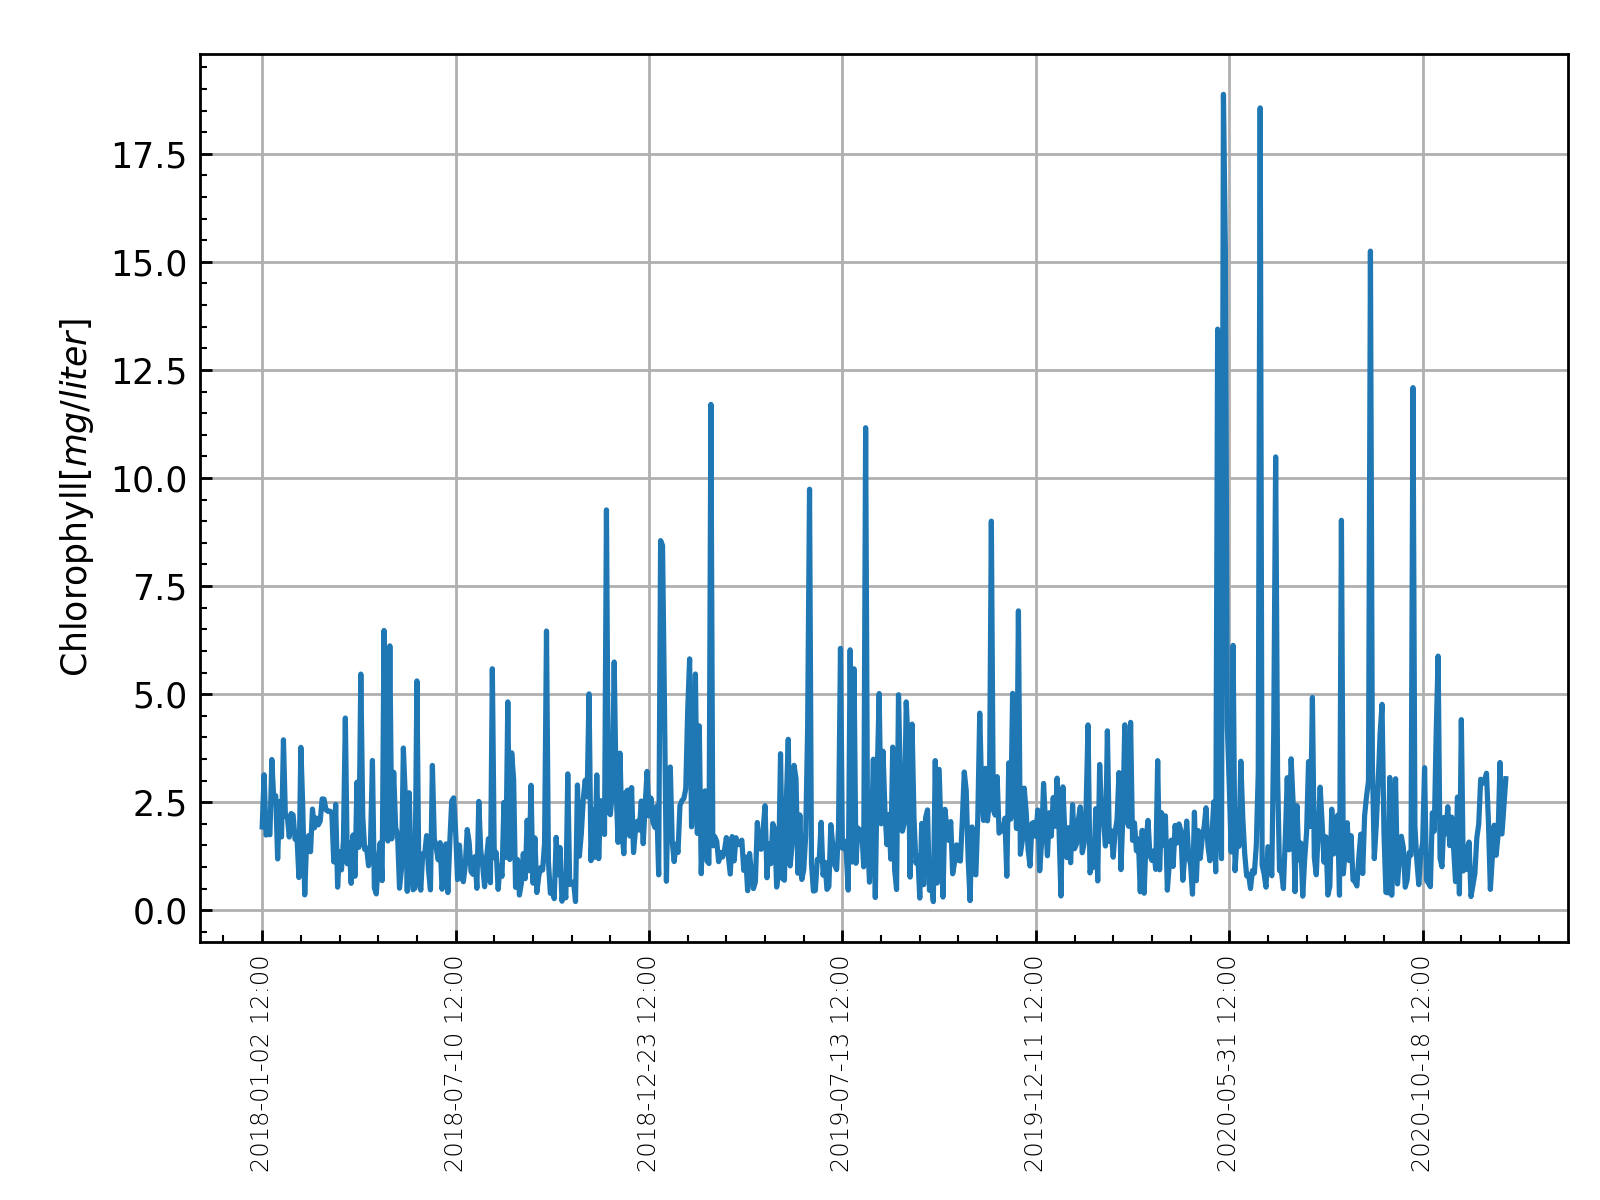
\includegraphics[scale=0.5]{figs/plots/chlor_a.png}}
    \label{fig:aqua_sst}
    \caption{AQUA-MODIS}
\end{figure}

\subsection{Verification}
    By plotting a correlation matrix between the field sea temperature and MODIS sea surface temperature we can make sure they are consistent with each other thus reduceing the possibility of an error.    
we verify our correlation of in-situ measured temperature and remotely observed SST.

\begin{figure}[H]
    \centering
    \subfloat[In-situ sea temperature vs MODIS SST]{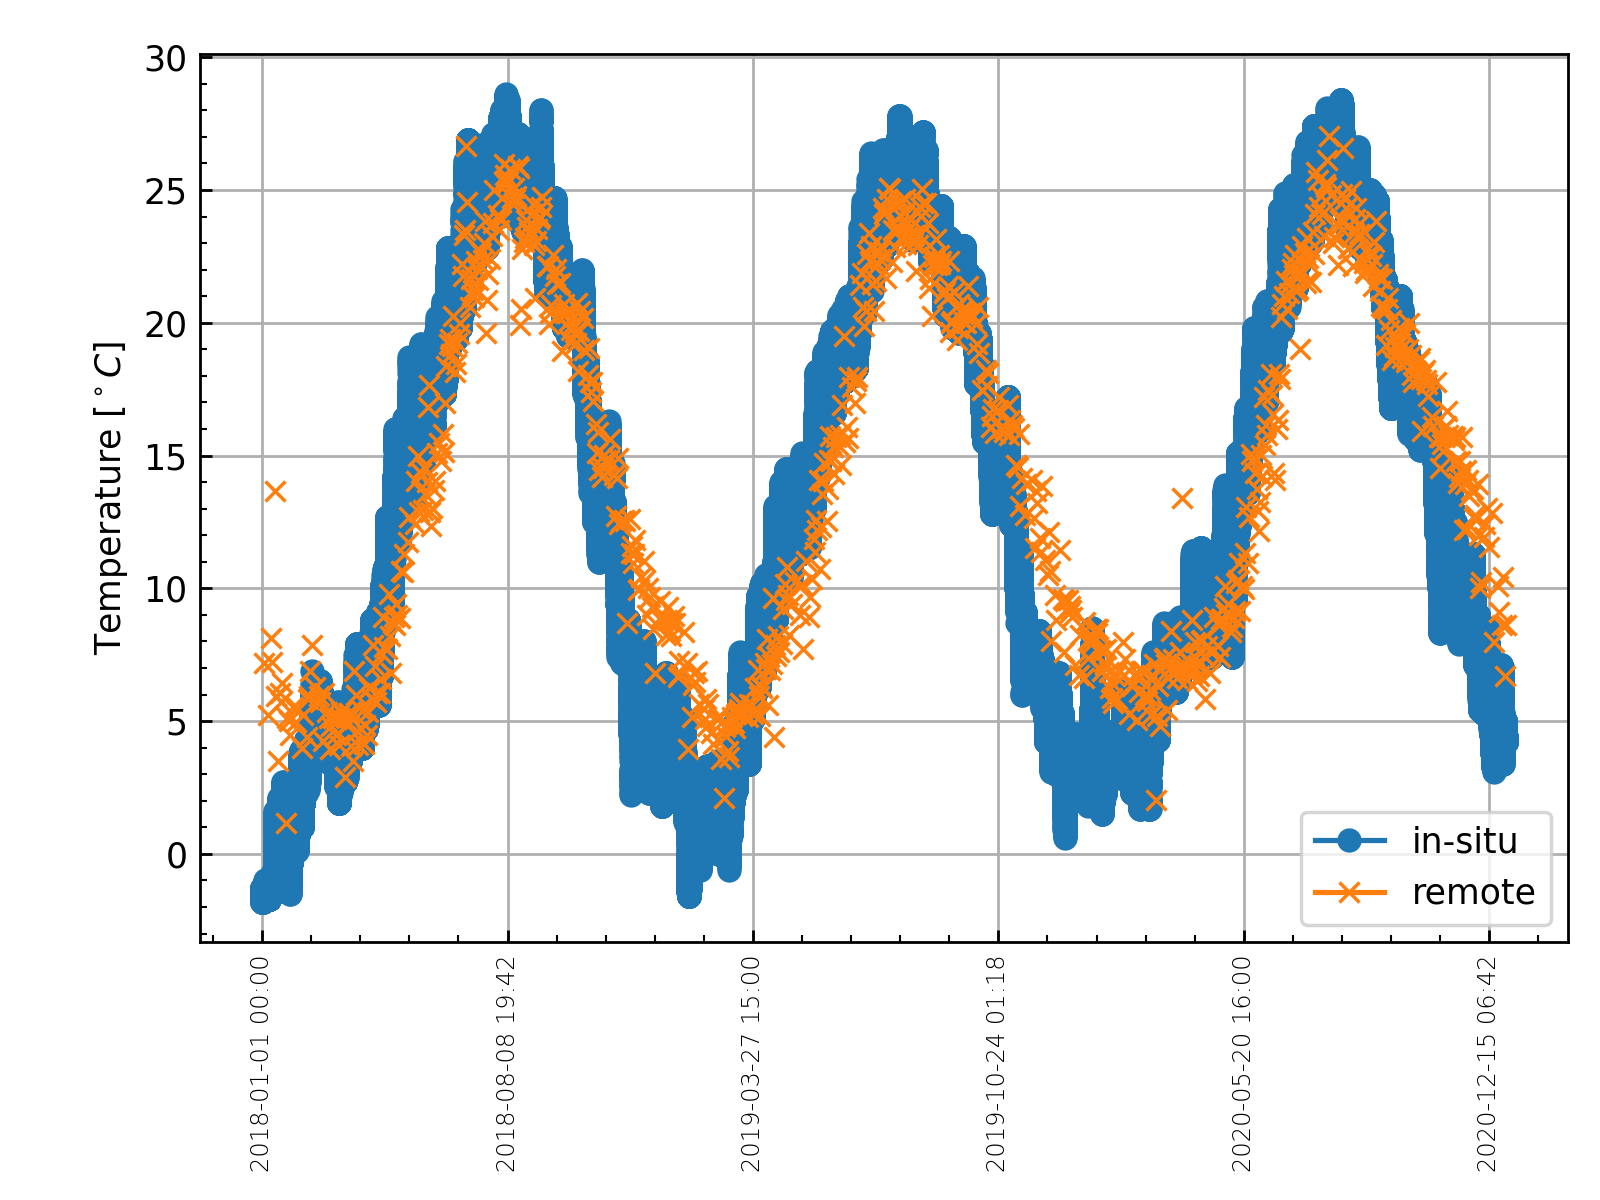
\includegraphics[scale=0.55]{figs/plots/temp_vs_sst.png}}
    \quad
    \subfloat[Correlation matrix]{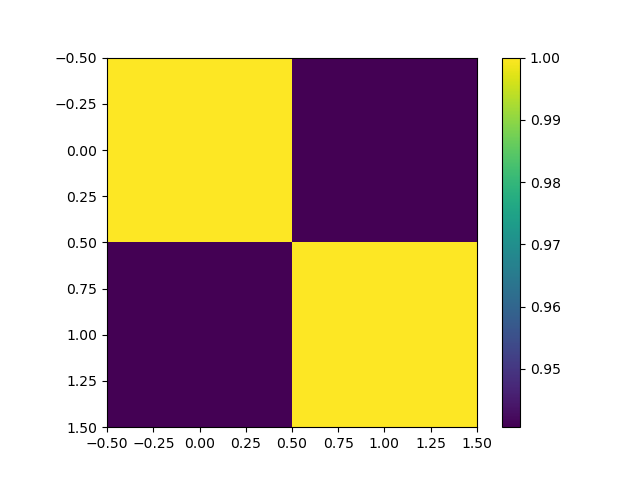
\includegraphics[scale=0.4]{figs/plots/temp_vs_sst_corr.png}}
    \caption{Verification of in-situ temperature and AQUA-MODIS SST($11\mu m$)}
\end{figure}

\begin{figure}[H]
    \centering
    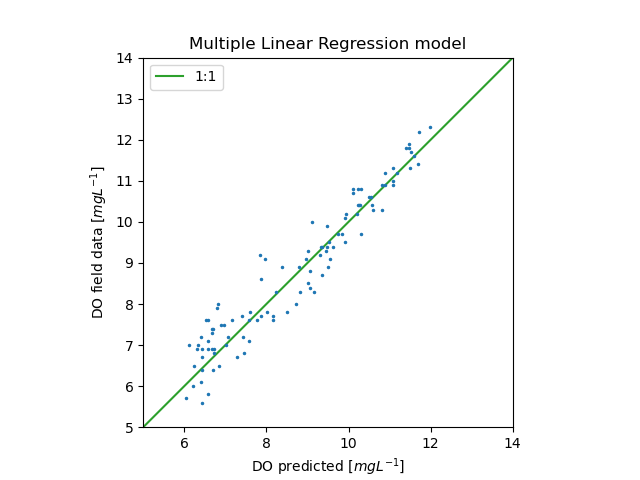
\includegraphics[scale=1.0]{figs/plots/mlr_test.png}
    \caption{Model test}
\end{figure}

Fig.17 suggests a good correlation with predictions and test labels of the data. We find that there is 24\% error associated with our predictions which could be reduced by using more longer and vivid datasets.
        % \subsection{Data extraction}
        % \subsection{Multiple Regression model}
        % \subsection{Model accuracy}
    \section{Conclusion}
        \paragraph{}
    In this study, DO measurements of Orient NY monitoring station and MODIS data was used to develop and validate the multiple linear regression model.

    As discussed in section III, the MLR model predicts with adequate accuracy which could be improved by adding data from multiple sources with multiple water characteristics.

    All codes for extraction and processing of data are available at \href{https://github.com/devanshshukla99/Analysis-of-DO}{devanshshukla99/Analysis-of-DO}.
    
    \section{References}
        \begin{enumerate}
    \item Y. H. Kim, S. Son, H.-C. Kim, B. Kim, Y.-G. Park, J. Nam, and J. Ryu, “Application
        of satellite remote sensing in monitoring dissolved oxygen variabilities: A case study for
        coastal waters in korea,” Environment International, vol. 134, p. 105301, 2020. [Online].
        Available: https://www.sciencedirect.com/science/article/pii/S0160412019327291
    \item NASA Ocean Biology Processing Group. (2018). MODIS-TERRA Level 3 Mapped Chlorophyll Data Version R2018.0 [Data set]. NASA Ocean Biology DAAC. https://doi.org/10.5067/TERRA/MODIS/L3M/CHL/2018
    \item R. F. Keeling, A. K¨ortzinger, and N. Gruber, “Ocean deoxygenation in a warming world,”
    Annual Review of Marine Science, vol. 2, no. 1, pp. 199-229, 2010, pMID: 21141663.
    [Online]. Available: https://doi.org/10.1146/annurev.marine.010908.163855
    \item K. Triana and A. J. Wahyudi, “Dissolved oxygen variability of indonesian seas over
    decades as detected by satellite remote sensing,” IOP Conference Series: Earth and
    Environmental Science, vol. 925, no. 1, p. 012003, nov 2021. [Online]. Available:
    https://doi.org/10.1088/1755-1315/925/1/012003
    \item M. H. Gholizadeh, A. M. Melesse, and L. Reddi, “A comprehensive review on water quality
    parameters estimation using remote sensing techniques,” Sensors (Switzerland), vol. 16, 8
    2016
    \item Chi, L., Song, X., Yuan, Y., Wang, W., Cao, X., Wu, Z., Yu, Z., 2020. Main factors 
    dominating the development, formation and dissipation of hypoxia off the 
    Changjiang Estuary (CE) and its adjacent waters, China. Environ. Pollut. https://doi. 
    org/10.1016/j.envpol.2020.
    \item Schulzweida, Uwe. (2021, October 31). CDO User Guide (Version 2.0.0). Zenodo. http://doi.org/10.5281/zenodo.5614769
\end{enumerate}

    % \bibliographystyle{IEEEtran}
    % \bibliography{IEEEabrv,citations.bib}
    % \cite{*}
    % \bibliographystyle}
    % \bibliography{abbrvnat, citations.bib}

\end{document}